
\documentclass[xcolor=dvipsnames]{beamer}  % for hardcopy add 'trans'

\mode<presentation>
{
  \usetheme{Singapore}
  % or ...
  \setbeamercovered{transparent}
  % or whatever (possibly just delete it)
}

\usefonttheme{professionalfonts}
%\usepackage[english]{babel}
% or whatever
%\usepackage[latin1]{inputenc}
% or whatever
%\usepackage{times}
%\usepackage[T1]{fontenc}
% Or whatever. Note that the encoding and the font should match. If T1
% does not look nice, try deleting the line with the fontenc.

%%%%%%%%%%%%%%%%%%%%%% start my preamble %%%%%%%%%%%%%%%%%%%%%%


\addtobeamertemplate{navigation symbols}{}{%
    \usebeamerfont{footline}%
    \usebeamercolor[fg]{footline}%
    \hspace{1em}%
    \insertframenumber/\inserttotalframenumber
}

\setbeamercolor{footline}{fg=blue}
\setbeamerfont{footline}{series=\bfseries}


%\usepackage{epsfig}
\usepackage{graphicx}
\usepackage{amsmath, amssymb, amsthm}

\usepackage{fancyvrb}

\usepackage{tikz}
\usetikzlibrary{arrows}
\usetikzlibrary{calc}
\usetikzlibrary{intersections}
\usetikzlibrary{decorations}
\usepackage{pgf}
\usepackage{pgfplots}
\pgfplotsset{compat=1.13}

\usepackage{graphviz}
 
\usepackage{verbatim}


\usepackage{algorithmicx,algpseudocode}


%font
\usepackage{mathpazo}
%\usepackage[usenames, dvipsnames]{color}

%\usepackage[linesnumbered, ruled, lined]{algorithm2e}

\usepackage{xr}
\externaldocument[ET-]{et}


\newcommand*{\theorembreak}{\usebeamertemplate{theorem end}\framebreak\usebeamertemplate{theorem begin}}

\newcommand{\newtopic}[1]{\textcolor{Green}{\Large \bf #1}}
\newcommand{\navy}[1]{\textcolor{Blue}{\bf #1}}
\newcommand{\navymth}[1]{\textcolor{Blue}{#1}}
\newcommand{\red}[1]{\textcolor{red}{#1}}


\definecolor{pale}{RGB}{235, 235, 235}
\definecolor{pale2}{RGB}{175,238,238}
\definecolor{turquois4}{RGB}{0,134,139}

% Typesetting code
\definecolor{bg}{rgb}{0.95,0.95,0.95}
\usepackage{minted}
\usemintedstyle{friendly}
\newminted{python}{mathescape,frame=lines,framesep=4mm,bgcolor=bg}
\newminted{ipython}{mathescape,frame=lines,framesep=4mm,bgcolor=bg}
\newminted{julia}{mathescape,frame=lines,framesep=4mm,bgcolor=bg}
\newminted{c}{mathescape,linenos=true}
\newminted{r}{mathescape,  frame=none, baselinestretch=1, framesep=2mm}
\renewcommand{\theFancyVerbLine}{\sffamily
    \textcolor[rgb]{0.5,0.5,1.0}{\scriptsize {\arabic{FancyVerbLine}}}}


\usepackage{stmaryrd}

\newcommand{\Fact}{\textcolor{Brown}{\bf Fact. }}
\newcommand{\Facts}{\textcolor{Brown}{\bf Facts }}
\newcommand{\keya}{\textcolor{turquois4}{\bf Key Idea. }}
\newcommand{\Factnodot}{\textcolor{Brown}{\bf Fact }}
\newcommand{\Eg}{\textcolor{ForestGreen}{Example. }}
\newcommand{\Egs}{\textcolor{ForestGreen}{Examples. }}
\newcommand{\Ex}{{\bf Ex. }}
\newcommand{\Thm}{\textcolor{Brown}{\bf Theorem. }}
\newcommand{\Prf}{\textcolor{turquois4}{\bf Proof.}}
\newcommand{\Ass}{\textcolor{turquois4}{\bf Assumption.}} 
\newcommand{\Lem}{\textcolor{Brown}{\bf Lemma. }}

%source code 



% caligraphic
\usepackage{mathrsfs}
\usepackage{bbm}
\usepackage{subfigure}

\newcommand{\argmax}{\operatornamewithlimits{argmax}}
\newcommand{\argmin}{\operatornamewithlimits{argmin}}

\newcommand\T{{\mathpalette\raiseT\intercal}}
\newcommand\raiseT[2]{\raisebox{0.25ex}{$#1#2$}}

\DeclareMathOperator{\cl}{cl}
%\DeclareMathOperator{\argmax}{argmax}
\DeclareMathOperator{\interior}{int}
\DeclareMathOperator{\Prob}{Prob}
\DeclareMathOperator{\kernel}{ker}
\DeclareMathOperator{\diag}{diag}
\DeclareMathOperator{\sgn}{sgn}
\DeclareMathOperator{\determinant}{det}
\DeclareMathOperator{\trace}{trace}
\DeclareMathOperator{\Span}{span}
\DeclareMathOperator{\rank}{rank}
\DeclareMathOperator{\cov}{cov}
\DeclareMathOperator{\corr}{corr}
\DeclareMathOperator{\range}{rng}
\DeclareMathOperator{\var}{var}
\DeclareMathOperator{\mse}{mse}
\DeclareMathOperator{\se}{se}
\DeclareMathOperator{\row}{row}
\DeclareMathOperator{\col}{col}
\DeclareMathOperator{\dimension}{dim}
\DeclareMathOperator{\fracpart}{frac}
\DeclareMathOperator{\proj}{proj}
\DeclareMathOperator{\colspace}{colspace}

\providecommand{\inner}[1]{\left\langle{#1}\right\rangle}

% mics short cuts and symbols
% mics short cuts and symbols
\newcommand{\st}{\ensuremath{\ \mathrm{s.t.}\ }}
\newcommand{\setntn}[2]{ \{ #1 : #2 \} }
\newcommand{\cf}[1]{ \lstinline|#1| }
\newcommand{\otms}[1]{ \leftidx{^\circ}{#1}}

\newcommand{\fore}{\therefore \quad}
\newcommand{\tod}{\stackrel { d } {\to} }
\newcommand{\tow}{\stackrel { w } {\to} }
\newcommand{\toprob}{\stackrel { p } {\to} }
\newcommand{\toms}{\stackrel { ms } {\to} }
\newcommand{\eqdist}{\stackrel {\textrm{ \scriptsize{d} }} {=} }
\newcommand{\iidsim}{\stackrel {\textrm{ {\sc iid }}} {\sim} }
\newcommand{\1}{\mathbbm 1}
\newcommand{\dee}{\,{\rm d}}
\newcommand{\given}{\, | \,}
\newcommand{\la}{\langle}
\newcommand{\ra}{\rangle}

\renewcommand{\rho}{\varrho}

\newcommand{\htau}{ \hat \tau }
\newcommand{\hgamma}{ \hat \gamma }

\newcommand{\boldx}{ {\mathbf x} }
\newcommand{\boldu}{ {\mathbf u} }
\newcommand{\boldv}{ {\mathbf v} }
\newcommand{\boldw}{ {\mathbf w} }
\newcommand{\boldy}{ {\mathbf y} }
\newcommand{\boldb}{ {\mathbf b} }
\newcommand{\bolda}{ {\mathbf a} }
\newcommand{\boldc}{ {\mathbf c} }
\newcommand{\boldi}{ {\mathbf i} }
\newcommand{\bolde}{ {\mathbf e} }
\newcommand{\boldp}{ {\mathbf p} }
\newcommand{\boldq}{ {\mathbf q} }
\newcommand{\bolds}{ {\mathbf s} }
\newcommand{\boldt}{ {\mathbf t} }
\newcommand{\boldz}{ {\mathbf z} }

\newcommand{\boldzero}{ {\mathbf 0} }
\newcommand{\boldone}{ {\mathbf 1} }

\newcommand{\boldalpha}{ {\boldsymbol \alpha} }
\newcommand{\boldbeta}{ {\boldsymbol \beta} }
\newcommand{\boldgamma}{ {\boldsymbol \gamma} }
\newcommand{\boldtheta}{ {\boldsymbol \theta} }
\newcommand{\boldxi}{ {\boldsymbol \xi} }
\newcommand{\boldtau}{ {\boldsymbol \tau} }
\newcommand{\boldepsilon}{ {\boldsymbol \epsilon} }
\newcommand{\boldmu}{ {\boldsymbol \mu} }
\newcommand{\boldSigma}{ {\boldsymbol \Sigma} }
\newcommand{\boldOmega}{ {\boldsymbol \Omega} }
\newcommand{\boldPhi}{ {\boldsymbol \Phi} }
\newcommand{\boldLambda}{ {\boldsymbol \Lambda} }
\newcommand{\boldphi}{ {\boldsymbol \phi} }

\newcommand{\Sigmax}{ {\boldsymbol \Sigma_{\boldx}}}
\newcommand{\Sigmau}{ {\boldsymbol \Sigma_{\boldu}}}
\newcommand{\Sigmaxinv}{ {\boldsymbol \Sigma_{\boldx}^{-1}}}
\newcommand{\Sigmav}{ {\boldsymbol \Sigma_{\boldv \boldv}}}

\newcommand{\hboldx}{ \hat {\mathbf x} }
\newcommand{\hboldy}{ \hat {\mathbf y} }
\newcommand{\hboldb}{ \hat {\mathbf b} }
\newcommand{\hboldu}{ \hat {\mathbf u} }
\newcommand{\hboldtheta}{ \hat {\boldsymbol \theta} }
\newcommand{\hboldtau}{ \hat {\boldsymbol \tau} }
\newcommand{\hboldmu}{ \hat {\boldsymbol \mu} }
\newcommand{\hboldbeta}{ \hat {\boldsymbol \beta} }
\newcommand{\hboldgamma}{ \hat {\boldsymbol \gamma} }
\newcommand{\hboldSigma}{ \hat {\boldsymbol \Sigma} }

\newcommand{\boldA}{\mathbf A}
\newcommand{\boldB}{\mathbf B}
\newcommand{\boldC}{\mathbf C}
\newcommand{\boldD}{\mathbf D}
\newcommand{\boldI}{\mathbf I}
\newcommand{\boldL}{\mathbf L}
\newcommand{\boldM}{\mathbf M}
\newcommand{\boldP}{\mathbf P}
\newcommand{\boldQ}{\mathbf Q}
\newcommand{\boldR}{\mathbf R}
\newcommand{\boldX}{\mathbf X}
\newcommand{\boldU}{\mathbf U}
\newcommand{\boldV}{\mathbf V}
\newcommand{\boldW}{\mathbf W}
\newcommand{\boldY}{\mathbf Y}
\newcommand{\boldZ}{\mathbf Z}

\newcommand{\bSigmaX}{ {\boldsymbol \Sigma_{\hboldbeta}} }
\newcommand{\hbSigmaX}{ \mathbf{\hat \Sigma_{\hboldbeta}} }

\newcommand{\RR}{\mathbbm R}
\newcommand{\CC}{\mathbbm C}
\newcommand{\NN}{\mathbbm N}
\newcommand{\PP}{\mathbbm P}
\newcommand{\EE}{\mathbbm E \nobreak\hspace{.1em}}
\newcommand{\EEP}{\mathbbm E_P \nobreak\hspace{.1em}}
\newcommand{\ZZ}{\mathbbm Z}
\newcommand{\QQ}{\mathbbm Q}


\newcommand{\XX}{\mathcal X}

\newcommand{\aA}{\mathcal A}
\newcommand{\fF}{\mathscr F}
\newcommand{\bB}{\mathscr B}
\newcommand{\iI}{\mathscr I}
\newcommand{\rR}{\mathscr R}
\newcommand{\dD}{\mathcal D}
\newcommand{\lL}{\mathcal L}
\newcommand{\llL}{\mathcal{H}_{\ell}}
\newcommand{\gG}{\mathcal G}
\newcommand{\hH}{\mathcal H}
\newcommand{\nN}{\textrm{\sc n}}
\newcommand{\lN}{\textrm{\sc ln}}
\newcommand{\pP}{\mathscr P}
\newcommand{\qQ}{\mathscr Q}
\newcommand{\xX}{\mathcal X}

\newcommand{\ddD}{\mathscr D}


\newcommand{\R}{{\texttt R}}
\newcommand{\risk}{\mathcal R}
\newcommand{\Remp}{R_{{\rm emp}}}

\newcommand*\diff{\mathop{}\!\mathrm{d}}
\newcommand{\ess}{ \textrm{{\sc ess}} }
\newcommand{\tss}{ \textrm{{\sc tss}} }
\newcommand{\rss}{ \textrm{{\sc rss}} }
\newcommand{\rssr}{ \textrm{{\sc rssr}} }
\newcommand{\ussr}{ \textrm{{\sc ussr}} }
\newcommand{\zdata}{\mathbf{z}_{\mathcal D}}
\newcommand{\Pdata}{P_{\mathcal D}}
\newcommand{\Pdatatheta}{P^{\mathcal D}_{\theta}}
\newcommand{\Zdata}{Z_{\mathcal D}}




\newcommand{\e}[1]{\mathbbm{E}[{#1}]}
\newcommand{\p}[1]{\mathbbm{P}({#1})}

%\theoremstyle{plain}
%\newtheorem{axiom}{Axiom}[section]
%\newtheorem{theorem}{Theorem}[section]
%\newtheorem{corollary}{Corollary}[section]
%\newtheorem{lemma}{Lemma}[section]
%\newtheorem{proposition}{Proposition}[section]
%
%\theoremstyle{definition}
%\newtheorem{definition}{Definition}[section]
%\newtheorem{example}{Example}[section]
%\newtheorem{remark}{Remark}[section]
%\newtheorem{notation}{Notation}[section]
%\newtheorem{assumption}{Assumption}[section]
%\newtheorem{condition}{Condition}[section]
%\newtheorem{exercise}{Ex.}[section]
%\newtheorem{fact}{Fact}[section]

% Bibliography
\usepackage[authordate,uniquename=false,firstinits,backend=biber,maxcitenames=2]{biblatex-chicago}
\DeclareFieldFormat[article]{title}{#1}
\DeclareFieldFormat[inproceedings]{title}{#1}
\addbibresource{et_newbib.bib}
\renewcommand{\cite}{\textcite}



\setlength{\parskip}{1.5ex plus0.5ex minus0.5ex}


\setlength{\jot}{12pt} 










\title{A Primer in Econometric Theory}

\subtitle
{Lecture 3: Foundations of Probability}

\author{John Stachurski \\ \tiny Lectures by Akshay Shanker}




\begin{document}

\begin{frame}
  \titlepage
\end{frame}

\section{Probabilistic Models}

\begin{frame}

    \vspace{2em}
    Probability fundamental to statistics and econometrics, but technically demanding:
    
    \begin{itemize}
        \item set of events we want to assign probabilities to can be very large 
        \item we need ways to manage the complexity 
    \end{itemize}
    
    \vspace{1em}
    Before we begin:
    \begin{itemize}
        \item a set $S$ is countable if it is finite or can be represented as sequence 
        \item otherwise, a set $S$ is uncountable
    \end{itemize}

\end{frame}

\begin{frame}\frametitle{Sample Spaces and Events}

    \vspace{2em}
    \navy{Sample space} can be thought of as a ``list" of
    all possible outcomes in a given random experiment:
    \begin{itemize}
        \item sample space usually denoted by $\Omega$
        \item sample space can be any non-empty set
        \item typical element of $\Omega$ is denoted $\omega$
   \end{itemize}
   
    \vspace{1em}
    A realization of uncertainty will lead to the selection of
    a particular $\omega\in \Omega$
    
\end{frame}


\begin{frame}

    \vspace{2em}
    \Eg
    In a random experiment that involves rolling a die once, the set of
    possible outcomes is naturally represented by $\Omega := \{1,\ldots, 6\}$
    
    \vspace{1em}
    \Eg
    \label{eg:dart}
    Burton Malkiel's blindfolded monkey throws darts at a
    dartboard of radius $1$
    
    Impose ordinary
    Cartesian coordinates with origin at the centre of the board
    
    Let $(h,
    v)$ be a typical location measured on the horizontal and vertical
    coordinates respectively
    
    A natural sample space is $\Omega :=
    \setntn{(h, v) \in \RR^2}{\| (h, v) \| \leq 1}$ -- also called
    the \navy{unit disk} in $\RR^2$
    
\end{frame}

\begin{frame}

    \vspace{2em}
    Informally, an \navy{event} is a subset of $\Omega$ (we will address some caveats soon)
    
    \vspace{1em}
    An event $A$
    occurs whenever the individual $\omega \in \Omega$ selected in the random
    experiment happens to lie in $A$
    
\end{frame}

\begin{frame}

    \vspace{2.5em}
    
    \begin{figure}
   \begin{center}
    \scalebox{.32}{\input{figs_code/event_occurs.pdf_t}}
    \caption{\label{f:eao} Outcomes and events}
   \end{center}
    \end{figure}

\end{frame}

\begin{frame}
    \frametitle{Probabilities and events}
    
    \vspace{2em}
    Can we assign probabilities to each $\omega\in \Omega$?
    
    Consider dart throwing model where $\Omega$ is $\mathbb{R}$:
    \begin{itemize}
        \item for $A\subset \Omega$, probability dart lands in $A$ is 
                proportional to the area of $A$
        \item the probability of a point $\omega \in \Omega$ will be less 
                than any area $A$ containing $\omega$
        \item for any $\epsilon>0$, we can find an $A$, containing $\omega$, 
                with area smaller than $\epsilon$
    \end{itemize}
    
    The probability of hitting $\omega$ is smaller than $\epsilon$ for 
    any $\epsilon >0$, thus the probability of hitting $\omega$ must be zero!
    
\end{frame}

\begin{frame}

    \vspace{2em}
    The upshot: when sample space is uncountable, assign probabilities to events (subsets of $\Omega$), 
    not to each $\omega\in \Omega$
    
    But can we assign probabilities to \emph{every} subset of $\Omega$? 
    
    In the dart model:
    \begin{equation*}
        \PP(A) = \frac{\lambda(A)}{\pi} 
    \end{equation*}
    
    where $\lambda(A)\colon = \text{area of the set A}$

\end{frame}

\begin{frame}

    \vspace{2em}
    Defining area of $A$, for all $A\subset \Omega$, problematic:
    
    \begin{itemize}
        \item the space $\Omega$, our dart-board unit disk in $\mathbb{R}^{2}$, 
        contains many subsets which exhibit strange phenomena
        \item Banach-Tarski paradox 
    \end{itemize}

    Solution: do not take the set of events to be all the subsets of $\Omega$
    
    Take the set of events to be certain ``well-behaved" subsets of $\Omega$, denoted by $\mathscr{F}$

    Assign probabilities only to subsets of $\Omega$ in $\mathscr{F}$

\end{frame}

\begin{frame}\frametitle{Sigma-algebra}

    \vspace{2em}
    How can we ensure $\mathscr{F}$ is large enough? In a sensible probability model, 
    we ideally want:
    \begin{itemize}
        \item the event ``not A" to belong to $\mathscr{F}$ if $A\in \mathscr{F}$
        \item the event ``A or B" to belong to $\mathscr{F}$ if $A\in \mathscr{F}$ 
                and $A\in \mathscr{F}$
    \end{itemize}
    
    \vspace{1em}
    Formally, $\fF$ is a
    \navy{$\sigma$-algebra} on $\Omega$ if
    %
    \begin{enumerate}
        \item $A \in \fF \implies A^c \in \fF$,
        \item $A_1, A_2, \ldots \in \fF \implies \cup_{n=1}^{\infty} A_n \in \fF$,
            and
        \item $\Omega \in \fF$
    \end{enumerate}
    
\end{frame}

\begin{frame}

    \vspace{2em}
    1. - 3. imply that $\emptyset \in \fF$ if $\fF$ is a $\sigma$-algebra
    
    The event $\emptyset$ is called the \navy{impossible event} 
    
    The event $\Omega$ is called the \navy{certain event}
    
    \vspace{1em}
    \Eg The set $\{\Omega, \emptyset\}$ is a $\sigma$ - algebra called 
    the \navy{trivial $\sigma$-algebra}
    
\end{frame}

\begin{frame}\frametitle{The Borel $\sigma$ -algebra}
    
    \vspace{2em}
    The $\sigma$-algebra of events varies from problem to problem
    
    In $\mathbb{R}^{N}$, we use the Borel sets, denoted by $\bB(\RR^N)$ 
    \begin{itemize}
        \item the smallest $\sigma$-algebra that contains all the rectangles in $\mathbb{R}^{N}$ 
    \end{itemize}
    
    Why  Borel $\sigma$-algebra?
    \begin{itemize}
        \item excludes ``strange" sets 
        \item includes day-to-day useful sets (including planes and
        hyperplanes, circles, spheres, polygons, finite sets, and sequences of points)
    \end{itemize}
    
\end{frame}

\begin{frame}\frametitle{Probabilities}

    \vspace{2em}
    For given event $B\in \fF$, the symbol
    $\PP(B)$ represents ``the probability that event $B$
    occurs."
    %
    \begin{quote}
        $\PP(B)$ represents the probability that
        when uncertainty is resolved and some $\omega \in \Omega$ is selected by
        ``nature,'' the statement $\omega \in B$ is true
    \end{quote}
    
\end{frame}

\begin{frame}

    \vspace{2em}
    We need to place restrictions to make probabilities well-behaved
    
    For example, we want to rule out $\PP(B) = -93$ for some $B$
    
    \vspace{1em}
    Let $\Omega$ be a nonempty set and let $\fF$ be a $\sigma$-algebra 
    of subsets of $\Omega$.  A \navy{probability} $\PP$ on $(\Omega, \fF)$
    is a function from $\fF$ to $[0,1]$ that satisfies
    %
    \begin{enumerate}
        \label{enum:prob}
      \item $\PP(\Omega) = 1$ and
      \item $\PP(\cup_{n=1}^{\infty} A_n) = \sum_{n=1}^{\infty} \PP(A_n)$ for any
          disjoint sequence of sets $A_1, A_2, \ldots \in \fF$
    \end{enumerate}
     
     $\PP$ is also called a \navy{probability measure}; 
     the triple $(\Omega, \fF, \PP)$ is called a \navy{probability space}
    
\end{frame}

\begin{frame}
    
    \vspace{2em}
    Axiom 1.: we require $\PP(\Omega) = 1$
    because, by construction, every possible $\omega$ lies in the set $\Omega$.

    Axiom 2. is called \navy{countable additivity}
    
    Disjointness
    in the statement of axiom (ii) is pairwise: any distinct pair $A_i, A_j$ share
    no points in common
    
    Countable additivity implies finite \navy{additivity}:
    %
    \begin{equation}
        \label{eq:add}
        \PP(A_1 \cup \cdots \cup A_k)
        = \PP (A_1) + \cdots + \PP (A_k)
    \end{equation}
    %
    whenever $A_1, \ldots, A_k$ are disjoint
    
\end{frame}

\begin{frame}
    
    \vspace{2em}
    \begin{figure}
       \begin{center}
        \scalebox{.23}{\input{figs_code/additivity.pdf_t}}
        \caption{\label{f:additivity} Each of the $N$ dots occurs with probability $1/N$}
       \end{center}
    \end{figure}
    %
    \begin{equation*}
    \PP(A \cup B \cup C) = \frac{9}{N}  
    = \PP(A) + \PP(B) + \PP(C)
    \end{equation*}

\end{frame}

\begin{frame}

    \vspace{2em}
    \Eg
    Let $\Omega := \{1,\ldots, 6\}$
    represent the six different faces of a die, as in example~\ref{ET-eg:ram00}
    
    
    Since $\Omega$ is finite, take $\fF$ to be the set of all
    subsets of $\Omega$
    
    Define a probability $\PP \colon \fF \to [0,1]$
    %
    \begin{equation}
        \label{eq:defpd}
        \PP(A) := \frac{|A|}{6}
        \quad \text{where } \, 
        |A| := \text{ number of elements in set $A$}
    \end{equation}
    %
    Easy to see $0 \leq \PP(A) \leq 1$ for
    any $A \in \fF$, and that $\PP(\Omega) = 1$

\end{frame}

\begin{frame}
    
    \vspace{2em}
    \Eg (cont.)
    Regarding additivity,
    suppose $A$ and $B$ are two disjoint subsets of $\{1,\ldots, 6\}$
    
    Then $|A \cup B| = |A| + |B|$, hence
    %
    \begin{equation*}
        \PP(A \cup B) 
         = \frac{|A \cup B|}{6} 
         = \frac{|A| + |B|} {6}
         = \frac{|A|}{6} + \frac{|B|}{6}
         = \PP(A) + \PP(B)
    \end{equation*}


    This proves additivity for pairs of sets.  An analogous argument confirms
    additivity for any finite collection
    
    Finite additivity is in this case equivalent to countable additivity,
    since the total number of distinct events is finite
    
\end{frame}

\begin{frame}

    \vspace{2em}
    \begin{example}
        A memory chip is made up of billions of tiny switches/bits

        \begin{itemize}
            \item Switches can be off or on (zero or 1)
        \end{itemize}
        
        Random number generator accesses $N$ bits, switching each one on or
        off

        We take 
        %
        \begin{itemize}
            \item $\Omega := \setntn{ (b_1,\ldots, b_N) } { \text{where } b_n
                \text{ is 0 or 1 for each } n}$
            \item $\PP(A) := 2^{-N} (\# A)$
        \end{itemize}
        
        Exercise: Show that $\PP$ is a probability
        
    \end{example}

\end{frame}


\begin{frame}

    \vspace{2em}
    \Eg     Consider again the dartboard model, where
    $\Omega$ is the unit disk in $\RR^2$
    
    For the event space, we take $\fF$ to be
    the set of Borel subsets of $\RR^2$ that lie inside $\Omega$
    
    For $\PP$ we
    follow the ``uniform" probability assignment given
    
    That is, $\PP(B) = \lambda(B) / \pi$ for every $B \in \fF$
    
    The
    function $\lambda$ that assigns area to Borel sets is known to be
    countably additive, in that $\lambda(\cup_n A_n) = \sum_{n=1}^\infty
    \lambda(A_n)$ whenever these sets are disjoint 
    
    Evidently $\PP(\Omega) = 1$

\end{frame}

\begin{frame}\frametitle{Lebesgue Measure}

        \vspace{2em}
    The function $\lambda$ mapping Borel sets to
    their ``area" is formally known as the \navy{Lebesgue measure}
    
    \S\ref{ET-ss:measure} in ET provides a brief introduction to this concept
    
\end{frame}

\begin{frame}\frametitle{Properties of Probability Measure}
    
    \vspace{2em}
    \Fact\eqref{ET-fa:bpro}
    Let $(\Omega, \fF, \PP)$ be a probability space,  and let $A, B \in \fF$\
    
    If $A \subset B$, then
    %
    \begin{enumerate}
        \item $\PP(B \setminus A) = \PP(B) - \PP(A)$,
        \item $\PP(A) \leq \PP(B)$ (\navy{monotonicity})
        \item $\PP(A^c) = 1 - \PP(A)$, and
        \item $\PP(\emptyset) = 0$.
    \end{enumerate}
     
    \Prf
    When $A \subset B$, we have $B = (B \setminus A) \cup A$ and hence
    %
    \begin{equation*}
        \PP(B) = \PP(B \setminus A) + \PP(A)
    \end{equation*}
    %
    All results follow (why?)
    
\end{frame}
    
\begin{frame}

    \vspace{2em}
    \Fact\eqref{ET-fa:bpro2}
	If $A$ and $B$ are any (not necessarily disjoint) events, then
    %
    \begin{equation*}
        \PP(A \cup B) = \PP(A) + \PP(B) - \PP(A \cap B)       
    \end{equation*}
    %
    Proof as exercise \ref{ET-ex:bpro2} in ET

    Fact implies \navy{subadditivity}: for any $A, B \in \fF$, we have 
    %
    \begin{equation*}
        \PP(A \cup B) \leq \PP(A) + \PP(B)
    \end{equation*}
    
\end{frame}

\begin{frame}\frametitle{Conditional Probability and Independence}

    \vspace{2em}
    \navy{Conditional probability of $A$ given $B$} is 
    %
    \begin{equation}
      \label{eq:efcp}
      \PP(A \,|\, B) := \frac{\PP(A \cap B)}{\PP(B)}
    \end{equation}
    %
    Probability of $A$, given information that $B$ has occurred

\end{frame}

\begin{frame}

    \vspace{2em}
    Events $A$ and $B$ called \navy{independent} if $\PP(A \cap B) = \PP(A) \PP(B)$
    
    \begin{itemize}
        \item If $A$ and $B$ independent, then 
            %
            \begin{equation*}
                \PP(A \,|\, B) 
                := \frac{\PP(A \cap B)}{\PP(B)} 
                = \frac{\PP(A) \PP(B)}{\PP(B)} 
                = \PP(A)
            \end{equation*}
            
    \end{itemize}
    
\end{frame}


\begin{frame}

    \vspace{2em}
    \Eg
        Experiment: roll a dice twice  
        %
        \begin{equation*}
            \Omega := \setntn{(i, j)}{ i, j \in \{1,\ldots,6\}}
            \quad \text{and} \quad
            \PP(E) := \# E / 36
        \end{equation*}
        %
        Now consider the events 
        %
        \begin{equation*}
            A := \setntn{(i, j) \in \Omega}{i \text{ is even}}
            \quad \text{and} \quad
            B := \setntn{(i, j) \in \Omega}{j \text{ is even}}
        \end{equation*}
        %
        In this case we have
        %
        \begin{equation*}
            A \cap B = \setntn{(i, j) \in \Omega}{i \text{ and } j  \text{ are even}}
        \end{equation*}
        %
        Exercise: Verify that $\PP(A \cap B) = \PP(A) \PP(B)$

        Hence, $A$ and $B$ are independent under the probability $\PP$
        
\end{frame}

\begin{frame}\frametitle{Law of Total Probability}

    \vspace{2em}
    The \navy{Law of total probability} states:
    
    \Fact\eqref{ET-fa:ltp}
    If $A \in \fF$ and $B_1,\ldots, B_M$ is a partition of $\Omega$ with
    $\PP(B_m) > 0$ for all $m$, then
    %
    \begin{equation*}
      \PP(A) = \sum_{m=1}^M \PP(A \, | \, B_m) \cdot \PP(B_m)
    \end{equation*}
    %
    \Prf
        Given $A \in \fF$ and partition $B_1,\ldots, B_M$:
        %
        \begin{multline*}
            \PP(A) = \PP[A \cap (\cup_{m=1}^M B_m) ]
              = \PP[\cup_{m=1}^M (A \cap B_m)] \\
              = \sum_{m=1}^M \PP(A \cap B_m) 
              = \sum_{m=1}^M \PP(A \,|\, B_m) \cdot \PP(B_m)
        \end{multline*}
        %
\end{frame}

\begin{frame}\frametitle{Bayes' Law}
    
    \vspace{2em}
    \navy{Bayes law}: for any events $A$ and $B$ with positive
    probability, we have
    %
    \begin{equation}
        \label{eq:bt}
        \PP(A \given B) = \frac{\PP(B \given A) \PP(A)}{\PP(B)}
    \end{equation}
    \Prf 
    From the definition of conditional probability:
    %
    $$
        \PP(A \given B)=\frac{\PP(A \cap B)}{\PP(B)}
        \quad \text{and} \quad
        \PP(B \given A) = \frac{\PP(A \cap B)}{\PP(A)}
    $$
    Hence
        $\PP(A \cap B) = \PP(A \given B)\, \PP(B) = \PP(B \given A)\, \PP(A)$
    
    Rearranging yields \eqref{eq:bt}
    
\end{frame}

\begin{frame}

    \vspace{2em}
    \Eg
    Banks use automated systems to detect fraudulent or illegal
    transactions
    
    Consider test that responds to each transaction with $P$
    or $N$:
    \begin{itemize}
        \item $P$ means ``positive" (transaction flagged as fraudulent)
        \item $N$ means ``negative" (transaction flagged as normal)
    \end{itemize}
    
    Let $F$ mean fraudulent, suppose
    %
    \begin{itemize}
        \item $\PP( P \given F) = 0.99$ (the test flags 99\% of fraudulent
            transactions),
        \item $\PP( P \given F^c ) = 0.01$ (rate of false positives), and
        \item $\PP( F ) = 0.001$  (prevalence of fraud)
    \end{itemize}
    %
\end{frame}

\begin{frame}

    \vspace{2em}
    What is the probability of fraud given a positive test?
    
    Note Bayes' law
    %
    $$
        \PP(F \,|\, P) = \frac{\PP(P \given F)\PP(F)}{\PP(P)}
    $$
    and note the law of total probability 
        $$
        \PP(P) = \PP(P \given F) \PP(F) + \PP(P \given F^c) \PP(F^c)
        $$
    Hence
    %
    $$
        \PP(F \,|\, P) 
        = \frac{0.99 \times 0.001}{0.99 \times 0.001 + 0.01 \times 0.999}
        = \frac{11}{122}
        \approx \frac{1}{11}
    $$
    
\end{frame}

\section{Random Variables}

\begin{frame}

    \vspace{2em}
    \frametitle{Random variables}

    Informally: A ``value that changes randomly'' 
    
    Formally: A \navy{random variable} $x$ is a function from $\Omega$ into $\RR$
    
    Interpretation: random variables convert outcomes in sample space into
    numerical outcomes

    General idea: 
    %
    \begin{itemize}
        \item``nature''  picks out $\omega$ in $\Omega$ 
        \item random variable reports outcome as $x(\omega) \in \RR$
    \end{itemize}    
    
\end{frame}

\begin{frame}

    \vspace{2em}
    \Eg
        Suppose $\Omega$ is set of infinite binary sequences
        %
        \begin{equation*}
            \Omega := \setntn{(b_1, b_2, \ldots)}
                {b_n \in \{0, 1\} \text{ for each } n}
        \end{equation*}
        %
        We can create different random variables mapping $\Omega \to \RR$:
        %
        \begin{itemize}
            \item number of ``flips'' till first ``heads'':
                %
                \begin{equation*}
                    x(\omega) = x(b_1, b_2, \ldots) = \min \setntn{n}{b_n = 1}
                \end{equation*}
                %
            \item number of ``heads'' in first 10 ``flips'':
                %
                \begin{equation*}
                    x(\omega) = x(b_1, b_2, \ldots) = \sum_{n=1}^{10} b_n 
                \end{equation*}
                %
        \end{itemize}
        
\end{frame}


\begin{frame}

    \vspace{2em}
    \begin{itemize}
        \item number of flips until the first heads:
        %
        \begin{equation*}
            x(\omega) = x(b_1, b_2, \ldots) = \min \setntn{n \in \NN}{b_n = 1}
        \end{equation*}
        
        \item \navy{Binary or Bernoulli random variable} telling us whether 
        any heads occur in the first 10 flips:
        %
        \begin{equation}
            \label{eq:egbin}
            x(\omega) = y(b_1, b_2, \ldots) 
            := \min \left\{ \sum_{n=1}^{10} b_n , 1 \right\}
        \end{equation}
    
        \end{itemize}
        
        
\end{frame}


\begin{frame}\frametitle{Bernoulli Random Variable}

    \vspace{2em}
    \navy{Bernoulli} or \navy{binaary random variable} RVs $x$ take on values in $\{0,1\}$ 
    
    We now a consider generic way to create a Bernoulli RV
    
    Let $Q$ be a statement, such as ``$a$ is greater than 3'' 

    Definition: $\1\{Q\}$ equals one if $Q$ true, zero otherwise
    %
\end{frame}

\begin{frame}

    \vspace{2em}
    Define 
    \begin{equation*}
        x(\omega) = \1\{\omega \in A\}
        \;\;
        \text{ where } A \in \fF
    \end{equation*}
    %
    %
    The RV indicates whether or not event $C$ occurs  
    
    A common variation on
    the notation: for arbitrary $A \in \fF$:
    %
    \begin{equation*}
        \1_A(\omega) 
        := \1\{\omega \in A\} 
        := 
        \begin{cases}
            1 & \text{if } \omega \in A
            \\
            0 & \text{otherwise}
        \end{cases}
    \end{equation*}
    
\end{frame}

\begin{frame}

    \vspace{2em}
    \Fact\eqref{ET-fa:cbif}
    If $A_1, \ldots, A_N$ are subsets of $\Omega$, then
    %
    \begin{enumerate}
        \item $\1_{\cap_{n=1}^N A_n} = \prod_{n=1}^N \1_{A_n}$ and
        \item $\1_{\cup_{n=1}^N A_n } = \sum_{n=1}^N \1_{A_n}$
            whenever the sets are disjoint
    \end{enumerate}
    %
    See
    exercise~\ref{ET-ex:cbif} for proof 
    
    Here, equality means evaluated at any $\omega \in \Omega$
    
\end{frame}

\begin{frame}\frametitle{Notational Conventions}

    \vspace{2em}
    Common notational convention with RVs:
    %
    \begin{equation*}
        \{ x \text{ has some property} \} :=
        \setntn{\omega \in \Omega}{x(\omega) \text{ has some property}}
    \end{equation*}
    %

    \Eg 
    %
    \begin{equation*}
        \{x \leq 2\} := \setntn{\omega \in \Omega}{x(\omega) \leq 2}
    \end{equation*}
    %
    \vspace{1em}
    %
    \begin{equation*}
        \fore
        \PP\{x \leq 2\} := \PP\setntn{\omega \in \Omega}{x(\omega) \leq 2}
    \end{equation*}
    %
\end{frame}

\begin{frame}

    \vspace{2em}
    \Eg Given random variable $x$ and $a \leq b$, we claim
    %
    \begin{equation*}
        \label{eq:exno}
        \PP\{x \leq a\} \leq \PP\{x \leq b\}
    \end{equation*}
    %
    This holds because
    %
    \begin{multline*}
            \{x \leq a\} 
            := \setntn{\omega \in \Omega}{x(\omega) \leq a} \\
            \subset \setntn{\omega \in \Omega}{x(\omega) \leq b} 
            := \{x \leq b\}
    \end{multline*}
    %
    Now apply monotonicity: $A \subset B \implies \PP(A) \leq \PP(B)$
    
\end{frame}

\begin{frame}

    \vspace{2em}
    Equalities, inequalities and arithmetic operations should be
    interpreted \emph{pointwise}:
        %
    \begin{itemize}
        \item $x \leq y \; \iff \; x(\omega) \leq y(\omega)$ for all $\omega \in
        \Omega$,
        \item $x = y \; \iff \; x(\omega) = y(\omega)$ for all $\omega \in
        \Omega$, and
        \item $z = \alpha x + \beta y \; \iff \; z(\omega) = \alpha x(\omega) +
            \beta y(\omega)$ for all $\omega \in \Omega$
    \end{itemize}

\end{frame}

\begin{frame}\frametitle{Random Variables are Measurable Functions}

    \vspace{2em}
    Let $(\Omega, \fF, \PP)$ be any probability space
    
    Let $B$ be
    any subset of $\RR$
    
    Consider the probability
    %
    \begin{equation*}
        \PP\{x \in B\}
        := \PP\setntn{\omega \in \Omega}{x(\omega) \in B}
    \end{equation*}
    %
    Where $x$ is some function from $\Omega$ to $\RR$
    
    No way of being sure $\setntn{\omega \in \Omega}{x(\omega) \in B}$ is an element of
    $\fF$
    \begin{itemize}
        \item $\PP\{x \in B\}$ may not be defined
    \end{itemize}
    
\end{frame}

\begin{frame}

    \vspace{2em}
    We need to place restrictions:
    \begin{itemize}
        \item For $B$, we naturally
    restrict attention to $\bB(\RR)$, the Borel subsets of $\RR$
        \item For $x$, we require $\{x \in B\} \in \fF$ whenever $B$ is a Borel set
    \end{itemize}
    
    Formal definition of a random variable:
    
    A \navy{random variable} on $(\Omega, \fF)$ is a function
    $x \colon \Omega \to \RR$ satisfying 
    %
    \begin{equation}
        \label{eq:dorv}
        \setntn{\omega \in \Omega}{x(\omega) \in B} \in \fF
        \quad \text{for all } B \in \bB(\RR)
    \end{equation}
    %
    These kinds of functions are also  called $\fF$-measurable functions
    
\end{frame}

\begin{frame}

    \vspace{2em}
    Pre-image notation: $x^{-1}(B)$ is all $\omega \in \Omega$ such that $x(\omega)
    \in B$
    
    Rewrite \eqref{eq:dorv} as 
    %
    \begin{equation*}
        x^{-1}(B) \in \fF \quad \text{for all } B \in \bB(\RR)
    \end{equation*}
    
    Thus $x$ ``pulls back" Borel sets to events
    
\end{frame}

\begin{frame}
    \frametitle{Measurable Transformations}
    
    \vspace{2em}
    We want to discuss some transformation of $x$
    
    For example, $y := e^x$.
    Is $y$ also a random variable? 
    
    Yes, provided transformation satisfies  Borel
    measurability
    
    \vspace{.7em}
    Formally, $f \colon \RR \to \RR$ is called 
    \navy{Borel measurable}, or \navy{$\bB$-measurable}, if
    %
    \begin{equation}
        \label{eq:bm}
        f^{-1}(B) \in \bB(\RR)
        \quad \text{for all } B \in \bB(\RR)
    \end{equation}
    
\end{frame}

\begin{frame}

    \vspace{2em}
    Class of $\bB$-measurable functions is vast: any continuous function,
    any increasing function, etc., etc.
    
    \vspace{1em}
    Suppose $f$ is $\bB$-measurable and that $x$
    is a random variable
    
    We have $\{y \in B\} \in \fF$ for all $B \in \bB(\RR)$ because
    %
    \begin{equation}
        \label{eq:byim}
        \{y \in B\} = \{f(x) \in B\} = \{x \in f^{-1}(B)\}
    \end{equation}
    
    Thus $y =f(x)$ is a random variable
    
\end{frame}
    
\section{Expectations}


\begin{frame}

    \frametitle{Expectations}
    
    \vspace{2em}
    We want to define expectations for an arbitrary RV $x$

    Roughly speaking, $\EE[x] :=$ the ``sum'' of all possible values of $x$,
    weighted by their probabilities.  

    ``Sum'' in quotes because may be over an infinite number of possibilities
    
    We take a modern, formal and rigorous approach to defining expectations

\end{frame}

\begin{frame}

    \vspace{2em}
    For finite random variables, given probability space $(\Omega, \fF, \PP)$ 
    and random variable $x$ 
    taking only finitely many distinct values $s_1, \ldots, s_J$,
    the \navy{expectation} of $x$ is defined as
    %
    \begin{equation}
        \label{eq:expec}
        \EE x = \sum_{j=1}^J s_j \, \PP\{x = s_j\}
    \end{equation} 
    
\end{frame}

\begin{frame}

    \vspace{2em}
    \Eg
    Let's apply this definition to the simplest possible case, which is a
    random variable $x$ satisfying $x(\omega) = \alpha$ for all $\omega \in
    \Omega$, where $\alpha$ is some constant scalar value.  In this case the
    sum in \eqref{eq:expec} has only one term, and 
    %
    \begin{equation*}
        \EE x
        = \alpha \PP\{x = \alpha\} 
        = \alpha \PP\setntn{\omega \in \Omega}{x(\omega) = \alpha} 
        = \alpha \PP(\Omega) 
        = \alpha
    \end{equation*}
    
\end{frame}

\begin{frame}

    \vspace{2em}
    \Eg
    To evaluate the expectation of a binary random variable $x$,
    we apply \eqref{eq:expec} to obtain
    %
    \begin{equation*}
        \label{eq:expbin}
        \EE x  = 1 \times \PP\{x=1\} + 0 \times \PP\{x = 0\} = \PP\{x=1\}
    \end{equation*}
    %
\end{frame}

\begin{frame}

    \vspace{2em}
    \Eg
    Consider $N$ flips of a fair coin
    
    The sample space is $\Omega := \{0, 1\}^N$, the
    events are $\fF :=$  all subsets of $\Omega$, and $\PP(A) := 2^{-N} |A|$ for
    all $A \in \fF$
    
    Let 
        $x(\omega) = x(b_1, \ldots, b_N) = \sum_{n=1}^N b_n$
        
    
    Observe first that $0
    \leq x \leq N$
    
\end{frame}

\begin{frame}
    
    \vspace{2em}
    By the definition of $\PP$, for any $k$ we have
    $\PP\{x = k\} = 2^{-N} |A_k|$, where
    %
    \begin{equation*}
         A_k :=
         \{x = k\}
         = \left\{
               (b_1, \ldots, b_N) \in \Omega
                \; : \;
                \sum_{n=1}^N b_n = k
           \right\}
    \end{equation*}
    %
    From combinatorics, $|A_k| =
    \binom{N}{k}$, where the right-hand side is the so-called \navy{binomial
    coefficient} for $N,k$, which satisfies
    $\sum_{k=0}^N k \binom{N}{k} = N 2^{N-1}$ for all $N$
    
    The expectation of $x$ is 
    %
    \begin{equation*}
        \EE x 
        = \sum_{k=0}^N k \, 2^{-N} |A_k|
        = 2^{-N} \sum_{k=0}^N k \, \binom{N}{k} 
        = \frac{N}{2}
    \end{equation*}
    %
\end{frame}


\begin{frame}

    \vspace{2em}
    For general $x$, approximate arbitrary random variables with finite random variables 
    
    \begin{figure}
   \begin{center}
       \scalebox{0.8}{\begin{tikzpicture}[
    scale=5,
    axis/.style={->, >=stealth'},
    important line/.style={thick},
    dashed line/.style={dashed, thin},
    every node/.style={color=black}
    ]
   % define simple function
   \coordinate(O) at (0,0);
   \coordinate (s1) at (0.25,0);
   \coordinate (s2) at (0.65,0);
   \coordinate (s3) at (-0.15,0);
   \coordinate (s4) at (0.25,0.4);
   \coordinate (s5) at (0.65,0.4);
   \coordinate (s6) at (0.65,0.8);
   \coordinate (s7) at (1.1,0.8);
   \coordinate (s8) at (0,0.7);
   \coordinate (s9) at (1.1,0.95);
   % axis
   \draw[axis] (O)  -- (1.1,0) node(xline)[below, xshift=-0.8cm] {$\Omega$};
   \draw[axis] (0,0) -- (0,1.1) node(yline)[above] {};
   % drawing simple function
   \draw[important line,blue]  (O) -- (s1);
   \draw[important line,blue]  (s4) -- (s5);
   \draw[important line,blue]  (s6) -- (s7) node[right] {$x_n$};
   % continuous rv
   \draw[thick, xshift=0cm] plot [smooth, tension=1] coordinates { (O) (s4) (s6) (s9)} node[right] {$x$};
   % dashed line
   \draw[dashed line] (s1) -- (s4);
   \draw[dashed line] (s5) -- (s6);
   %circles
   \node[circle, draw,thin,blue,fill=white!10, scale=0.25] at (s1){};
   \node[circle, draw,thin,blue,fill=white!10, scale=0.25] at (s5){};
   \node[fill=blue,circle,scale=0.25] at (s4){};
   \node[fill=blue,circle,scale=0.25] at (s6){};
\end{tikzpicture}

}
    \caption{\label{f:finite_rv_approx} Finite approximation to a general random variable}
   \end{center}
    \end{figure}
    
\end{frame}


\begin{frame}
    
    \vspace{2em}
    We can improve approximation without limit-- let $x_n$ take a larger 
    and larger number of distinct values
    
    Process gives sequence of \emph{finite} random variables $x_n$
    converging to $x$
    
    Define the expectation of $x$ as
    %
    \begin{equation*}
        \label{eq:extar}
        \EE x := \lim_{n \to \infty} \EE x_n
    \end{equation*}

\end{frame}

\begin{frame}
    
    \vspace{2em}
    $\EE x$ is also referred to as
    the \navy{Lebesgue integral} of $x$ with respect to $\PP$, with the
    alternative notation
        $\EE x = \int x(\omega) \PP(\diff \omega)$
    \index{Lebesgue integral}
    
    \vspace{1em}
    Does a sequence of approximating random variables exist? 
    Yes, See page 94 in ET and \cite{dudley2002real}, proposition~4.1.5
    
\end{frame}

\begin{frame}

    \vspace{2em}
    If $x$ takes on negative values, then write $x = x^{+} - x^{-1}$
    
    Where $x^{+}\colon = \max\{x,0\}$ and $x^{-} = \min\{x,0\}$
    
    Define expectation as
    \begin{equation*}
        \EE x \colon = \EE x^{+} - \EE x^{-}
    \end{equation*}

    \vspace{.7em}
    Restrict
    attention to \navy{integrable} random variables: all random
    variables $x$ such that $\EE |x| < \infty$
    \begin{itemize}
        \item we have $x^+ \leq |x|$ and $x^-
            \leq |x|$
        \item thus, $\EE x \colon = \EE x^{+} - \EE x^{-}$ well-defined (why?)
    \end{itemize}
    
\end{frame}

\begin{frame}\frametitle{Properties of Expectation}

    \vspace{2em}
    \Fact\eqref{ET-fa:exprop}
        Given any probability space $(\Omega, \fF, \PP)$, there exists a uniquely
        defined function $\EE$ that maps each integrable random variable $x$
        on $(\Omega, \fF, \PP)$ into a value
        %
        \begin{equation}
            \label{eq:ealm}
            \EE x = \int x(\omega) \PP(\diff \omega)
        \end{equation}
        %
        in $\RR$, called the \navy{expectation of $x$} under $\PP$.  The
        function has the following properties:
        %
        \begin{enumerate}
            \item $\EE \alpha = \alpha$ for all $\alpha \in \RR$
            \item $\EE \1_A = \PP(A)$ for all $A \in \fF$
            \item $x \leq y \implies \EE x \leq \EE y$
            \item $\EE [ \alpha x + \beta y ] = \alpha \EE x + \beta \EE y$ for
                all integrable $x, y$ and constants $\alpha, \beta$
        \end{enumerate}
        
\end{frame}

\begin{frame}

    \vspace{2em}
    To remind ourselves of the underlying probability measure $\PP$ we may
      write $\mathbb{E}_{\PP} x$ instead of $\EE x$
     
    \vspace{.7em}
    Note the expression $\EE \alpha$ understood as the expectation of a 
     constant random variable equal to $\alpha$
     \begin{itemize}
         \item Follows from 4. by letting $x = \1_{\Omega}$ and $\beta = 0$
     \end{itemize}
     
\end{frame}

\begin{frame}

    \vspace{2em}
    Exercise: Check 3. for $x(\omega) := \1\{\omega \in A\}$ and 
    $y(\omega) := \1\{\omega \in B\}$ 

    Hint: What does $x \leq y$ imply about $A$ and $B$?
    
    For further details and references of proofs of the above fact, see page 96 in ET
    
\end{frame}

\begin{frame}

    \vspace{2em}
    We now prove that if $x$ is a finite
    random variable with range $\{s_j\}_{j=1}^J$ and $h$ is 
    any $\bB$-measurable function,then
    %
    \begin{equation}
        \label{eq:exh0}
        \EE h(x) = \sum_{j=1}^J h(s_j) \PP\{x = s_j\}
    \end{equation}
    %
    First observe that $\sum_{j=1}^J \1\{x = s_j\} = 1$, and hence we can
    write $h(x)$ as 
    %
    \begin{equation*}
        h(x) 
        = h(x) \sum_{j=1}^J \1\{x = s_j\}  
        = \sum_{j=1}^J h(s_j) \1\{x = s_j\}
    \end{equation*}
    
\end{frame}

\begin{frame}
    
    \vspace{2em}
    Using linearity of expectations:
        $$\EE h(x) =  \sum_{j=1}^J h(s_j) \EE \1\{x = s_j\}$$
    
    Applying part 2. of fact~\ref{ET-fa:exprop} leads to \eqref{eq:exh0}
    
\end{frame}

\begin{frame}
    
    \vspace{2em}
    
    \navy{Chebyshev's inequality}:
    \Fact\eqref{ET-fa:chein}
        For any nonnegative random variable $x$ and any $\delta > 0$, we have
        %
        \begin{equation}
            \label{eq:chein0}
            \PP\{x \geq \delta \} \leq \frac{\EE x}{\delta}
        \end{equation}
        %   
    
    A common variation of Chebyshev's inequality is the bound
    %
    \begin{equation}
        \label{eq:chein}
        \PP\{|x| \geq \delta \} \leq \frac{\EE x^2}{\delta^2}
    \end{equation}
    
    
    See Exercise~\ref{ET-ex:chein} for proof
    
\end{frame}

\begin{frame}

    \frametitle{Moments and Co-Moments}
    
    \vspace{2em}
    
    Let $x$ be a random variable and let $k \in \NN$. If $x^k$ is integrable, then 
    %
    \begin{itemize}
        \item $\EE [x^k] $ is called the \navy{$k$th moment} of $x$
        \item $\EE [ (x - \EE x)^k]$ is called the \navy{$k$th central moment} of
            $x$
    \end{itemize}
    %
    If $\EE [ |x|^k ] = \infty$, then the $k$th moment is said not to exist. 
    For
    some random variables even the first moment does not exist
    
    \vspace{.7em}
    For others, every
    moment exists
    
    \Fact\eqref{ET-fa:ofinm}
    If the $k$th moment of $x$ exists, then so does the $j$th for all $j \leq k$
    
    Proof: Exercise~\ref{ET-ex:ofinm}

\end{frame}

\begin{frame}

    \vspace{2em}
    The \navy{Cauchy--Schwarz inequality for random variables}:

    \vspace{1em}
    \Fact\eqref{ET-fa:csrv}
        If $x$ and $y$ are random variables with finite second moment, then
        %
        \begin{equation}
            \label{eq:csrv}
            \left| \, \EE [xy] \, \right| \leq \sqrt{ \EE[x^2] \EE[y^2] }
        \end{equation}
        %
\end{frame}

\begin{frame}

    \vspace{2em}
    The second central moment of $x$ is called the \navy{variance} of $x$:
    %
    \begin{equation*}
        \var x := \EE [ (x - \EE x)^2 ]
    \end{equation*}
    %
    The \navy{standard deviation} of $x$:
    %
    \begin{equation*}
        \sigma_x := \sqrt{\var x}
    \end{equation*}
    %
    The \navy{covariance} of random variables $x$ and $y$:
    %
    \begin{equation*}
        \cov[x, y] := \EE [ (x - \EE x)(y - \EE y) ]
    \end{equation*}
    
\end{frame}

\begin{frame}

    \vspace{2em}
    \Fact\eqref{ET-eq:efav}
    %
    If $x$ and $y$ have finite second moments, then
    %
    \begin{enumerate}
        \item $\var x$ and $\cov[x, y]$ are finite
        \item $\var x = \EE [x^2] - [\EE x]^2$, and
        \item $\cov[x, y] = \EE [ xy] -\EE[x] \EE[y]$
    \end{enumerate}

    Part 1. follows from 2.--3., the Cauchy--Schwarz inequality  and
    fact~\ref{ET-fa:ofinm}
    
    Parts 2.--3. follow from linearity of $\EE$ and
    some simple manipulations

\end{frame}

\begin{frame}

    \vspace{2em}
    \Fact\eqref{ET-fa:vacov}
    If $x_1,\ldots,x_N$ are random variables and 
    $\alpha_0, \alpha_1,\ldots,\alpha_N$ are constant scalars, then
    %
    \begin{equation*}
        \var \left[ \alpha_0 + \sum_{n=1}^N \alpha_n x_n \right]
        =  \sum_{n=1}^N \alpha_n^2 \var[ x_n ]   
                + 2 \sum_{n < m} \alpha_n \alpha_m \cov[x_n, x_m] 
    \end{equation*}
    
    \vspace{1em}
    Some simple implications:
    %
    \begin{enumerate}
        \item $\var[\alpha + \beta x] = \beta^2 \var[x]$ and
        \item $\var[\alpha x + \beta y] = \alpha^2 \var[x] + \beta^2 \var[y] + 2
            \alpha \beta \cov[x,y]$.
    \end{enumerate}
    
\end{frame}

\begin{frame}

    \vspace{2em}
    The \navy{correlation} of $x$ and $y$:
    %
    \begin{equation*}
        \corr[x,y] := \frac{\cov[x,y]}{\sigma_x \, \sigma_y}
    \end{equation*}
    %
    If $\corr[x,y] = 0$,  $x$ and $y$ are \navy{uncorrelated}
    
    Positive correlation means that $\corr[x,y]$ is positive and negative
    correlation means that $\corr[x,y]$ is negative

    \Fact\eqref{ET-fa:acorr}
        Given any two random variables $x$, $y$ and positive constants $\alpha$,
        $\beta$, we have 
        %
        \begin{equation*}
            -1 \leq \corr[x,y] \leq 1 
            \quad \text{ and }\quad  
            \corr[\alpha x, \beta y] = \corr[x,y]
        \end{equation*}
        %
    The first part follows from fact~\ref{ET-fa:csrv}; the second is 
    algebra
    
\end{frame}

\begin{frame}

    \vspace{2em}
    \frametitle{Best Linear Predictors}
    Consider the problem of predicting the value of a random variable $y$
    given knowledge of the value of a second random variable $x$ 
    
    We seek a
    function $f$ such that $f(x)$ is close to $y$ on average
    
    To measure the
    latter, we will use \navy{mean squared error}, which amounts in this case to  
    %
    \begin{equation*}
        \EE [ (y - f(x))^2 ]
    \end{equation*}
    
\end{frame}

\begin{frame}

    \vspace{2em}
    In\S\ref{ET-ss:ce}, to obtain minimizer of the mean squared
    deviation over all functions of $x$, we choose 
    $$f(x) = \EE[y \given
    x]$$
    
    \vspace{.7em}
    Here we'll consider finding a good predictor of $y$ within 
    the class of ``linear'' functions
    %
    \begin{equation*}
        \label{eq:llrv}
        \llL := \{ \text{ all functions of the form } \ell(x) = \alpha + \beta x \}
    \end{equation*}
    
\end{frame}

\begin{frame}

    \vspace{2em}
    Consider:
    %
    \begin{equation}
        \label{eq:llsrf}
        \min_{\ell \in \, \llL} \EE[ (y - \ell(x))^2 ] 
        = \min_{\alpha, \beta \in \RR} \EE[ (y - \alpha - \beta x)^2 ] 
    \end{equation}
    
    \vspace{.7em}
    If $\alpha$ and $\beta$ solve \eqref{eq:llsrf}, then the function
    %
    \begin{equation}
        \label{eq:blpre}
        \ell^*(x) := \alpha^* + \beta^* x
    \end{equation}
    %
    is called the \navy{best linear predictor} of $y$ given $x$
    
\end{frame}

\begin{frame}

    \vspace{2em}
    \Eg\eqref{ET-eg:mktbeta}
    Relationship between returns on a given asset $R_a$ and returns
    on a market benchmark $R_m$ is called the \navy{beta} of the asset
    
    Measures
    exposure to systemic risk, as opposed to idiosyncratic risk specific to
    the asset
    
    \vspace{.7em}
    The beta of $R_a$ is often defined as the coefficient
    $\beta^*$ in the best linear prediction \eqref{eq:blpre} when $x$ is
    returns on the market benchmark and $y=R_a$
    
\end{frame}

\begin{frame}

    \vspace{2em}
    To solve \eqref{eq:llsrf}, expand the square on the right-hand side and
    use linearity of $\EE$ to write the objective function as
    %
    \begin{equation*}
        \psi(\alpha, \beta) 
        := \EE [y^2] - 2 \alpha \EE[y] - 2 \beta \EE[xy] + 2\alpha\beta \EE[x]
            + \alpha^2 + \beta^2 \EE[x^2]
    \end{equation*}
    %
    Computing the derivatives and solving the first-order conditions:
    %
    \begin{equation}
        \label{eq:slpp}
        \beta^* := \frac{\cov[x,y]}{\var[x]}
        \quad \text{and} \quad
        \alpha^* := \EE[y] - \beta^* \EE[x]
    \end{equation}
    %
    See ex.~\ref{ET-ex:ctmi}
    
\end{frame}

\section{Distributions}

\begin{frame}\frametitle{Distributions}

    \vspace{2em}
    Take a random variable $x$ on probability space $(\Omega, \mathscr{F}, \mathbb{P})$
    
    Probability of $x$ taking on value in Borel set $B$ 
    %
        $$\PP\{x\in B\}$$
    
    \vspace{1em}
    In practice, more convenient to represent the probability
    as a \emph{distribution} over $\mathbb{R}$ 
    
\end{frame}


\begin{frame}

    \vspace{2em}
    Specialise $\Omega$ to $\RR$ and take the set of 
    events over $\RR$ as $\mathscr{B}(\RR)$
    
    \begin{itemize}
        \item A probability measure defined over $\mathscr{B}(\RR)$
        is called a \navy{law} or \navy{distribution}
    \end{itemize}
    
    \vspace{1em}
    Formally, a distribution
    $P$ is a map from $\bB(\RR)$ to $[0, 1]$ such that 
    %
    \begin{enumerate}
            \label{enum:nu}
        \item $P(\RR) = 1$ and
        \item $P(\cup_{n=1}^{\infty} B_n) = \sum_{n=1}^\infty P(B_n)$ 
            for any disjoint sequence $\{B_n\}$
    \end{enumerate}
    
\end{frame}

\begin{frame}

    \vspace{2em}
    If there exists a Borel set $S$
    with $P(S) = 1$, then we say that $P$ is \navy{supported} on $S$
    
    \vspace{1em}
    Characterise distributions using a \navy{cumulative distributed function},
    or {\sc cdf}, which is any function $F \colon \RR \to [0, 1]$ satisfying
    %
    \begin{enumerate}
        \item monotonicity: $s \leq s'$ implies $F(s) \leq F(s')$,
        \item right-continuity: $F(s_n) \downarrow F(s)$ whenever $s_n \downarrow
            s$, and
        \item $\lim_{s \to -\infty} F(s) = 0$ and $\lim_{s \to \infty} F(s) = 1$.
    \end{enumerate}
    
\end{frame}

\begin{frame}

    \vspace{2em}
    C{\sc df}s and distributions on $\RR$ can be put in one-to-one correspondence
    
    A distribution $P$ is entirely characterized by the values of the function
    %
    \begin{equation}
        \label{eq:ntf}
        F(s) := P( (-\infty, s] )
        \qquad (s \in \RR)
    \end{equation}
    
    \vspace{1em}
    \Fact\eqref{ET-fa:cdf}
    The following statements are true:
    %
    \begin{enumerate}
        \item If $P$ is any distribution on $\RR$, then the function $F$ in
            \eqref{eq:ntf} is a {\sc cdf}.
        \item Given any {\sc cdf} $F$ on $\RR$, there exists exactly one
            distribution $P$ satisfying \eqref{eq:ntf}
    \end{enumerate}
    
\end{frame}

\begin{frame}

    \vspace{2em}
    For a full proof, see \cite{williams1991probability}, lemma~1.6,
    or \cite{dudley2002real}, theorem~9.1.1.
    
    Here let's restrict ourselves to showing the function $F$ in
    \eqref{eq:ntf} satisfies part 1. of the definition of a {\sc cdf}
    
    \begin{itemize}
        \item observe 
    $s \leq s'$ implies $(-\infty, s] \subset (-\infty, s']$
        \item recall $P(A)\leq P(B)$ if $A\subset B$ 
        \item we then have $P((-\infty, s]) \leq P((-\infty, s'])$
        and $F(s) \leq F(s')$ as claimed
    \end{itemize}
 
\end{frame}

\begin{frame}

    \vspace{2em}
    \Eg
    The \navy{univariate normal distributions} or \navy{Gaussian
        distributions} refer to the class of distributions identified by {\sc
    cdf}s
    of the form
    %
    \begin{equation*}
        F(s) =
        \frac{1}{\sqrt{2 \pi} \sigma}
        \int_{-\infty}^s
           \exp \left\{ - 
               \frac{(t - \mu)^2}{2\sigma^2} \right\} \diff t
       \qquad (s \in \RR)
    \end{equation*}
    %
    where $\mu \in \RR$ and $\sigma > 0$
    
    We represent the distribution
    associated with $(\mu, \sigma)$ by $\nN(\mu, \sigma^2)$
    
    The distribution
    $\nN(0, 1)$ is called the \navy{standard normal distribution}
    
    We use the symbol $\Phi$ for its {\sc cdf}
    
\end{frame}

\begin{frame}

    \begin{figure}
   \begin{center}
    \scalebox{.45}{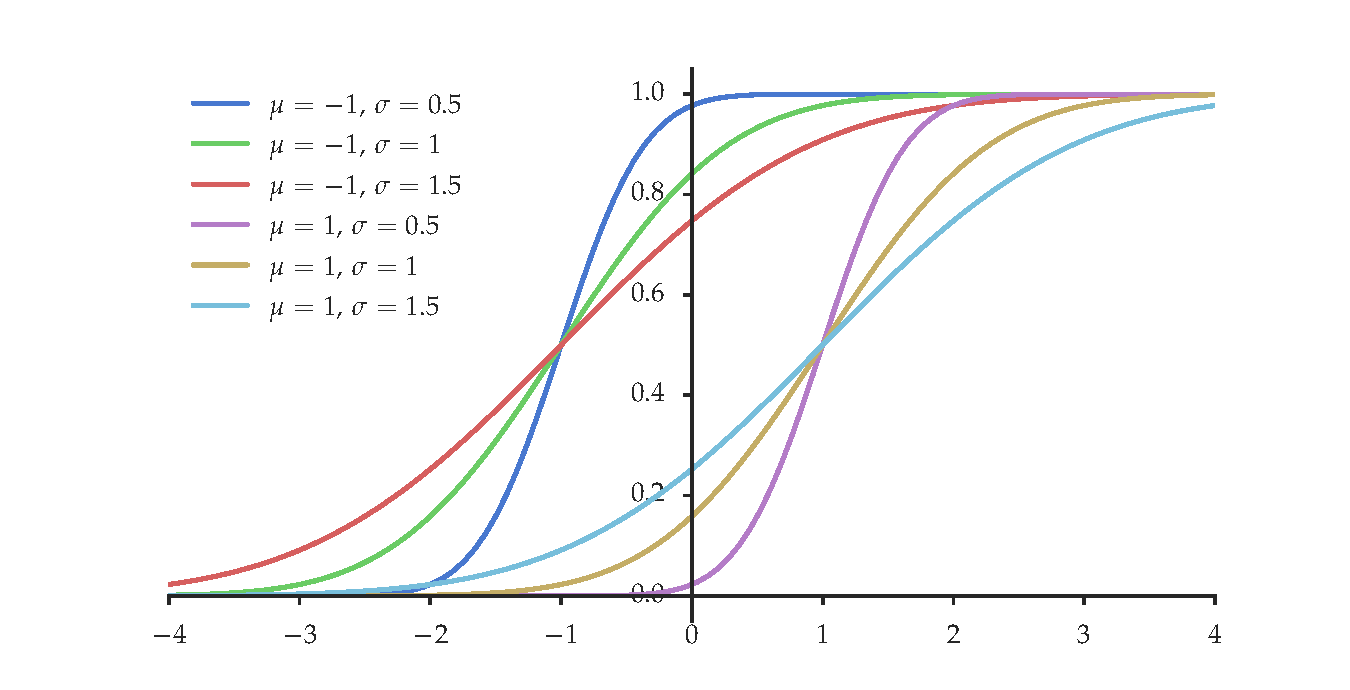
\includegraphics[trim={0 0em 0 2em}, clip]{normal_cdfs.pdf}}
    \caption{\label{f:normal_cdfs} Normal {\sc cdf}s }
   \end{center}
    \end{figure}
    
\end{frame}


\begin{frame}

    \vspace{2em}
    \Eg
    The \navy{Pareto distributions} are the univariate distributions
    with {\sc cdf}s of the form
    %
    \begin{equation*}
        F(s) = 
        \begin{cases}
            0   
                & \text{ if } s < s_0
            \\
            1 - \left(
                    \frac{s_0}{s}
                \right)^{\alpha} 
                & \text{ if } s_0 \leq s
        \end{cases}
        \qquad (s \in \RR, \; s_0, \, \alpha > 0)
    \end{equation*}
    %
    Pareto distributions often used to model phenomena with heavy right-hand tails, 
    such as the distribution of wealth or income

\end{frame}

\begin{frame}

    \vspace{2em}
    \Eg
    The class of \navy{beta {\sc cdf}s} is given by 
    %
    \begin{equation*}
        F(s) =
        \begin{cases}
            0 & \text{ if } s \leq 0
            \\
            \frac{1}{B(\alpha, \beta)}
                \int_0^s u^{\alpha-1} (1-u)^{\beta-1} \diff u
                & \text{ if } 0 < s < 1
            \\
            1   & \text{ if } 1 \leq s
        \end{cases}
    \end{equation*}
    %
    where $\alpha, \beta > 0$. 

    In this example $B(\alpha, \beta)$ is the \navy{beta function} 
    %
    \begin{equation*}
        B(\alpha, \beta) 
            := \frac{\Gamma(\alpha)\Gamma(\beta)}{\Gamma(\alpha + \beta)}
        \qquad \text{where} \qquad
        \Gamma(a) := \int_0^{\infty} u^{a-1} e^{-u} \diff u
    \end{equation*}
    %
    The function $\Gamma$ is called the \navy{gamma function}. 

\end{frame}

\begin{frame}
    
    \vspace{2em}
    \begin{figure}
       \begin{center}
        \scalebox{.45}{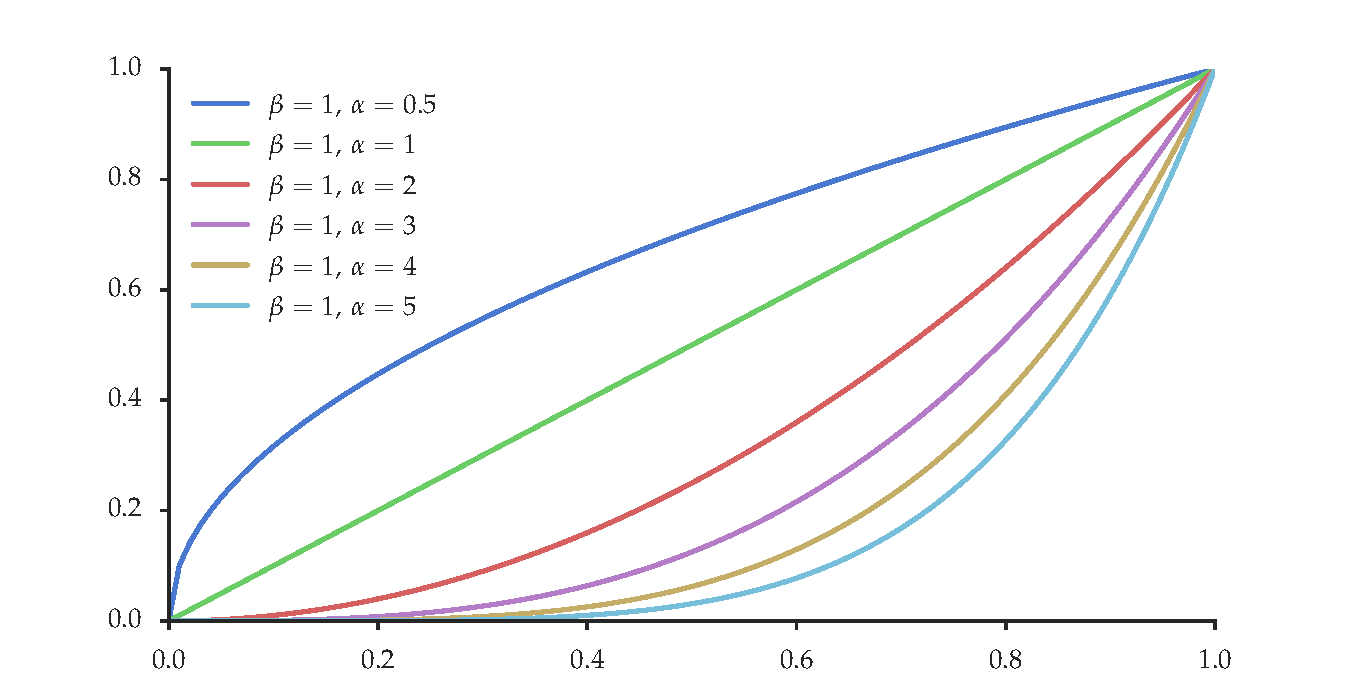
\includegraphics[trim={0 0em 0 3em}, clip]{beta_cdfs.pdf}}
        \caption{\label{f:beta_cdfs} Beta {\sc cdf}s }
       \end{center}
    \end{figure}

\end{frame}

\begin{frame}

    \Eg
    The class of \navy{Cauchy {\sc cdf}s} is given by 
    %
    \begin{equation*}
        F(s) 
        = \frac{1}{\pi} \arctan\left(  \frac{s - \tau}{\gamma} \right) 
            + \frac{1}{2}
       \qquad (s \in \RR)
    \end{equation*}
    %
    The parameters $\tau \in \RR$ and $\gamma > 0$ are the location
    and scale parameters respectively
    
    If $\tau=0$ and $\gamma=1$, then $F$ is called
    \navy{standard Cauchy}

\end{frame}

\begin{frame}

    \begin{figure}
       \begin{center}
        \scalebox{.45}{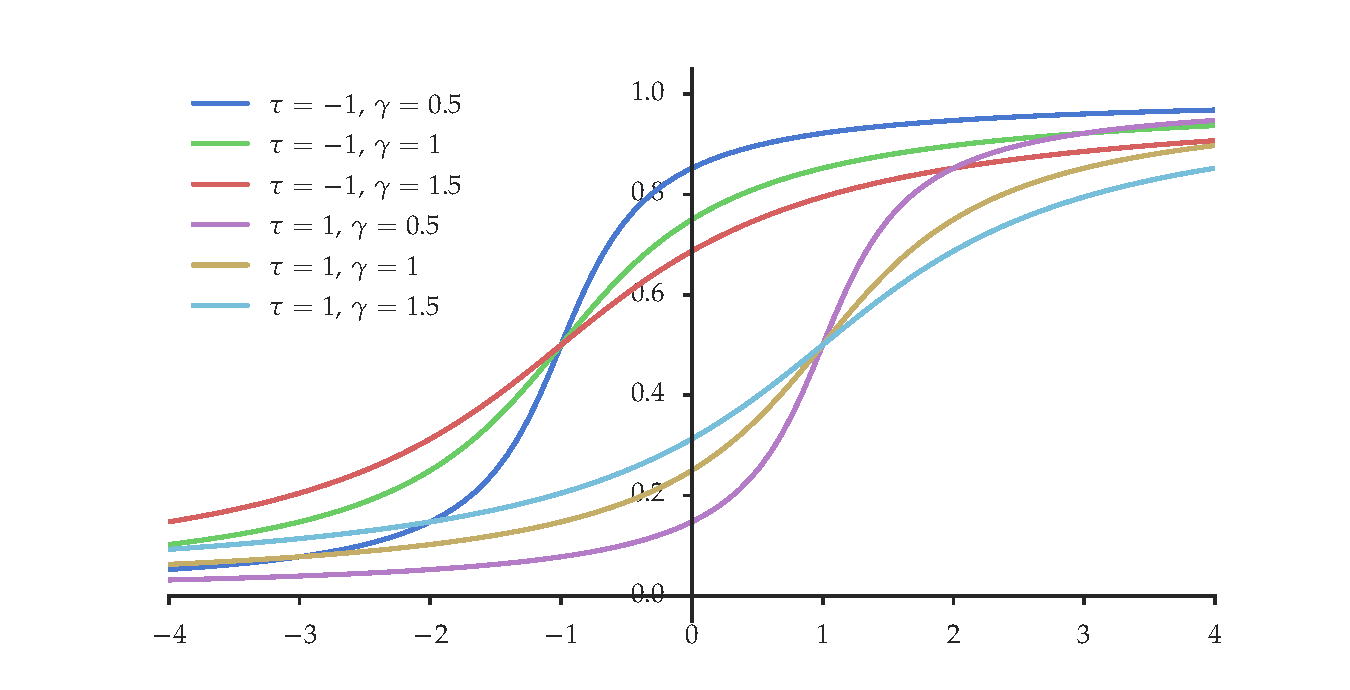
\includegraphics[trim={0 0em 0 3em}, clip]{cauchy_cdfs.pdf}}
        \caption{\label{f:cauchy_cdfs} Cauchy {\sc cdf}s }
       \end{center}
    \end{figure}
    
\end{frame}

\begin{frame}

    \vspace{2em}
    \Eg
    Given $a < b$, the \navy{uniform {\sc cdf}} on $[a, b]$ is the
    {\sc cdf} 
    %
    \begin{equation*}
        F(s) = 
        \begin{cases}
            0 & \text{ if } s \leq a
            \\
            \frac{s-a}{b-a} & \text{ if } a < s < b
            \\
            1   & \text{ if }  b \leq s
        \end{cases}
    \end{equation*}
    %
    We represent this distribution symbolically by $U[a, b]$
        
\end{frame}

\begin{frame}

    \frametitle{Densities and Probability Mass Functions}

    Two convenient special cases
    %
    \begin{itemize}
        \item discrete: CDF is just jumps (a step function) 
        \item absolutley continuous case: CDF smooth with no jumps
    \end{itemize}

\end{frame}

\begin{frame}\frametitle{Discrete Case}
    
    \vspace{2em}
    A distribution $P$ is called \navy{discrete} if it is supported on a countable
    set; that is, if there exists a countable set $\{s_j\}_{j \geq 1}$ with
    $P(\{s_j\}_{j \geq 1}) = 1$
    
    For such a $P$ let
    %
    \begin{equation*}
        p_j 
        := P\{s_j\} 
        := P(\{s_j\})
        = \text{probability mass on the single point } s_j
    \end{equation*}
    %
    A
    \navy{probability mass function}, or \navy{{\sc pmf}} is any non-negative
    sequence (finite or infinite) that sums to unity
    
    Exercise: show $\{p_j\}_{j \geq 1}$ is a
    \navy{probability mass function}
    
\end{frame}

\begin{frame}

    \vspace{2em}
    We can express the {\sc cdf} corresponding
    to $P$ as:
    %
    \begin{equation}
        \label{eq:cdfdrv}
        F(s) = \sum_{j \geq 1} \1\{s_j \leq s\} p_j
    \end{equation}
    %
    because
    %
    \begin{align*}
        F_x(s) := 
        \PP\{x \leq s\}
        & = \PP \bigcup_{j \st s_j \leq s} \{x = s_j\}
        \\
        & = \sum_{j \st s_j \leq s} \PP \{x = s_j\} 
        = \sum_{j=1}^J \1\{s_j \leq s\} p_j
    \end{align*}
    
\end{frame}

\begin{frame}

    \begin{figure}
       \begin{center}
        \begin{tikzpicture}[
    scale=5,
    axis/.style={->, >=stealth'},
    important line/.style={thick},
    dashed line/.style={dashed, thin},
    every node/.style={color=black},
    decoration={brace,amplitude=7pt},
    ]

    % define simple function
    \coordinate(O) at (0,0);
    \coordinate (s1) at (0.25,0);
    \coordinate (s2) at (0.65,0);
    \coordinate (s3) at (-0.15,0);
    \coordinate (s4) at (0.25,0.4);
    \coordinate (s5) at (0.65,0.4);
    \coordinate (s6) at (0.65,0.8);
    \coordinate (s7) at (1.1,0.8);
    % define curly bracket location
    \coordinate (c1) at (0.23,0.05); \coordinate (c2) at (0.23,0.35);
    \coordinate (c3) at (0.63,0.75); \coordinate (c4) at (0.63,0.45);
    % axis
    \draw[axis] (-0.15,0)  -- (1.1,0) node(xline)[below] {};
    \draw[axis] (0,0) -- (0,1.0) node(yline)[above] {};
    % drawing simple function
    \draw[important line,blue]  (s3) -- (s1);
    \draw[important line,blue]  (s4) -- (s5);
    \draw[important line,blue]  (s6) -- (s7);
    % dashed line
    \draw[dashed line] (s1) node[below] {$s_1$} -- (s4);
    \draw[dashed line] (s2) node[below] {$s_2$} -- (s6);
   % label y axis
   \foreach \y/\ytext in {0.8}
        \draw (0.0pt,\y cm) -- (-0.4pt,\y cm) node[anchor=east] {$1$};
   %curly bracket
   \draw [decorate,very thick] (c1) -- (c2)
   node [midway,anchor=east,inner sep=5pt, outer sep=5pt]{$p_1$};
   \draw [decorate,very thick] (c4) -- (c3)
   node [midway,anchor=east,inner sep=5pt, outer sep=5pt]{$p_2$};
   %circles
   \node[circle, draw,thin,blue,fill=white!10, scale=0.25] at (s1){};
   \node[circle, draw,thin,blue,fill=white!10, scale=0.25] at (s5){};
   \node[fill=blue,circle,scale=0.25] at (s4){};
   \node[fill=blue,circle,scale=0.25] at (s6){};
\end{tikzpicture}

        \caption{\label{f:discrete_cdf} Discrete {\sc cdf}}
       \end{center}
    \end{figure}

\end{frame}

\begin{frame}

    \vspace{2em}
    \Eg
    Given $N \in \NN$ and $\pi \in (0, 1)$, the sequence $\{p_0, \ldots,
    p_N\}$ defined by
    %
    $$
        p_j = {N\choose j}\pi^j(1-\pi)^{N-j}
    $$ 
    is called the \navy{binomial {\sc pmf}}
    
    The
    value $p_j$ is probability of $j$ successes in $N$ independent
    trials, each having success probability $\pi$

\end{frame}

\begin{frame}\frametitle{Absolutely Continuous Case}
    
    \vspace{2em}
    A \navy{density} is a nonnegative function $p$ on $\RR$ that integrates to 1
    
    \vspace{.7em}
    A distribution $P$ is \navy{represented by density $p$} (or \navy{has density $p$}) 
    if $p$ is a density and 
    %
    \begin{equation*}
        \label{eq:drbd}
        P(B) = \int_B p(s) \diff s
        \qquad \text{for all } B \in \bB(\RR)
    \end{equation*}
    %
    Note: 
    %
    \begin{equation*}
        \int_B p(s) \diff s := \int_{-\infty}^\infty \1_B(s) p(s) \diff s
    \end{equation*}
    
\end{frame}

\begin{frame}

    \vspace{2em}
    An exact necessary and
    sufficient condition for existence of density representation is absolute continuity
    
    \vspace{.7em}
    A
    distribution $P$ on the Borel subsets of $\RR$ is called \navy{absolutely
    continuous} if $P(B) = 0$ whenever $B$ has Lebesgue measure zero (see \S\ref{ET-ss:measure})
    \begin{itemize}
        \item Any countable subset of $\RR$ has Lebesgue measure zero
    \end{itemize}
    
    \vspace{2em}
    \Fact\eqref{ET-fa:denc}
        If $P$ is absolutely continuous, then $P(C) = 0$ whenever $C$ is
        countable
        
\end{frame}

\begin{frame}

    \vspace{2em}
    If distribution is absolutely continuous:
    
    \begin{itemize}
        \item individual points
    receive no probability mass 
        \item corresponding {\sc cdf} contains no jumps
        \item fundamental theorem of calculus says $F(s)$
        differentiable at all continuity points of $p$, and:
        %
        \begin{equation*}
            F'(s) = p(s)
            \qquad \text{for all } s \in \RR \text{ such that $p$  is continuous at $s$}
        \end{equation*}
    \end{itemize}
    
\end{frame}

\begin{frame}

    \vspace{2em}
    \Eg
    Normal {\sc cdf}s  are differentiable for all
    $\mu$, $\sigma$, with density
    %
    \begin{equation*}
        p(s) = F'(s) = 
        \frac{1}{\sqrt{2 \pi} \sigma}
           \exp \left\{ - 
               \frac{(s - \mu)^2}{2\sigma^2} \right\} 
    \end{equation*}
    %
    
    \vspace{.7em}
    We reserve the symbol $\phi$ for the
    standard normal density
    
\end{frame}

\begin{frame}

    \begin{figure}
   \begin{center}
    \scalebox{.45}{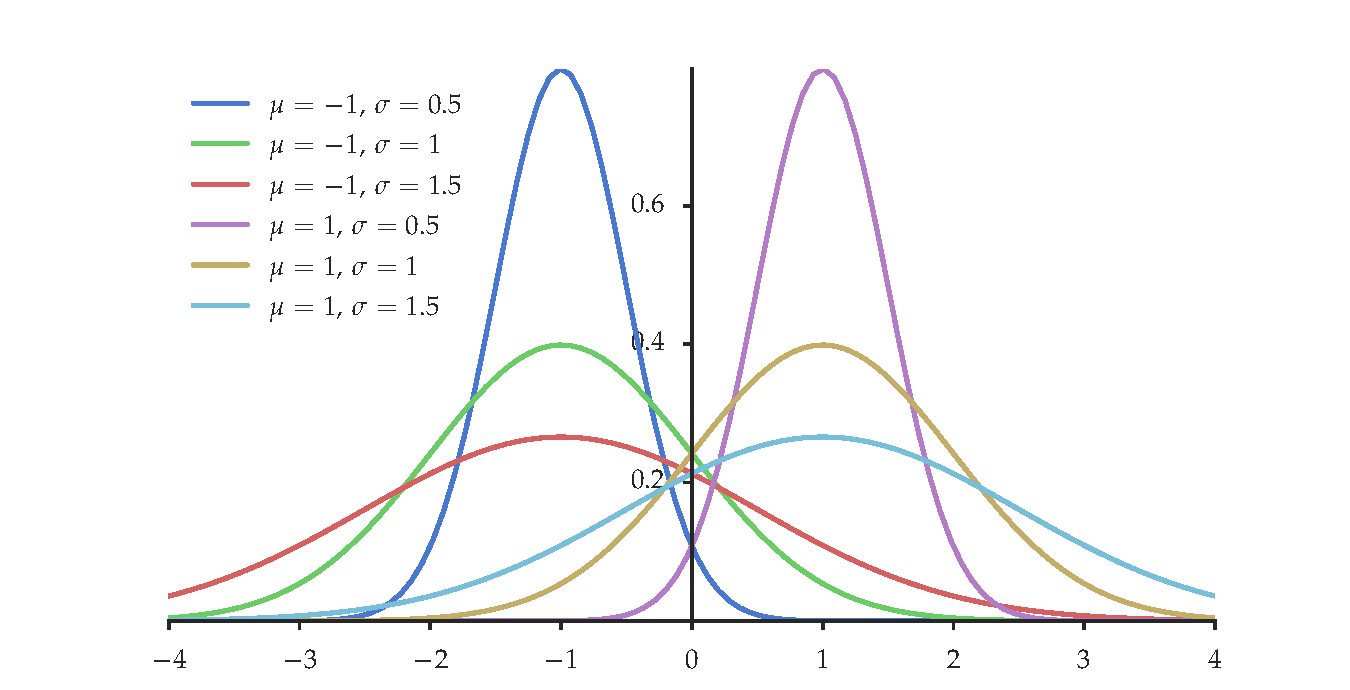
\includegraphics[trim={0 0em 0 2em}, clip]{normal_densities.pdf}}
    \caption{\label{f:normal_densities} Normal densities}
   \end{center}
    \end{figure}
    
\end{frame}

\begin{frame}

    \vspace{2em}
    \Eg
    The Cauchy {\sc cdf} has density
    %
    \begin{equation*}
        p(s) = 
        \frac{1}{\pi \gamma}
            \left[
                1 + \left( \frac{s - \tau}{\gamma} \right)^2
            \right]^{-1}
            \qquad (s \in \RR, \; \gamma > 0, \, \tau \in \RR)
    \end{equation*}
    %
    The Cauchy densities are more peaked around their modes and have greater
    mass in their tails than normal densities
    
\end{frame}

\begin{frame}

    \begin{figure}
   \begin{center}
    \scalebox{.45}{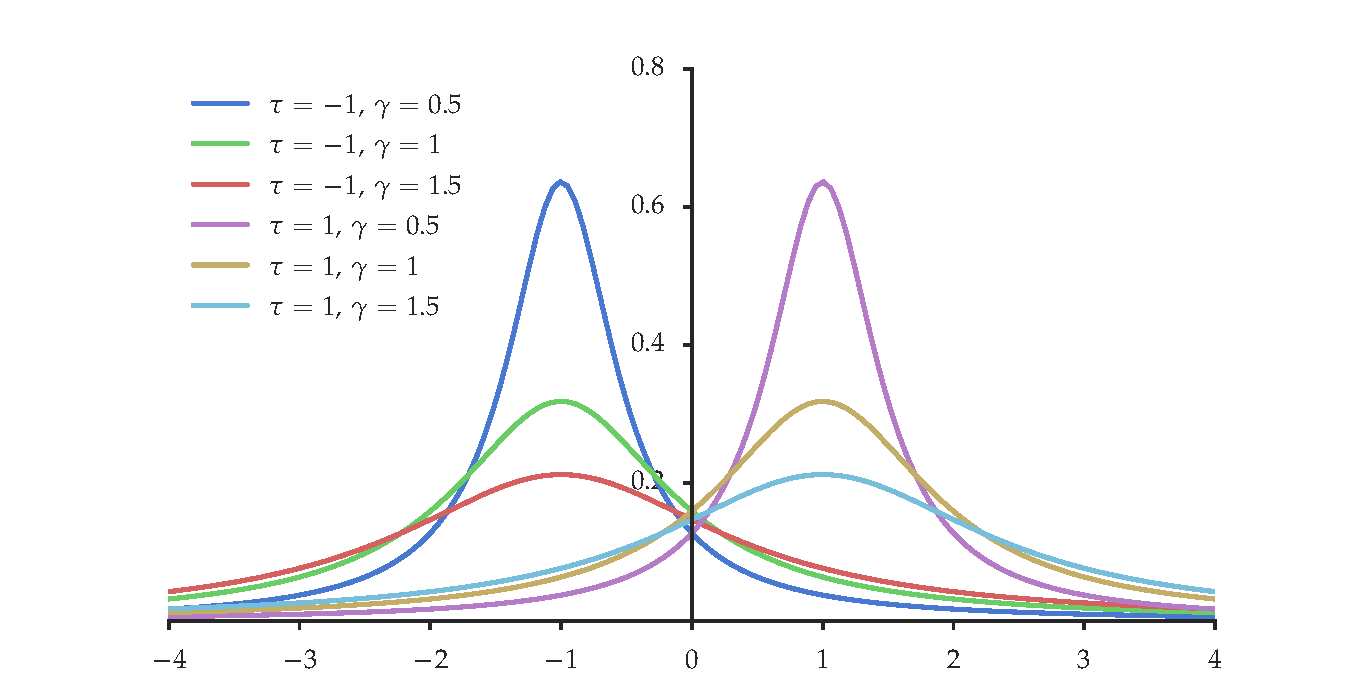
\includegraphics[trim={0 0em 0 2em}, clip]{cauchy_densities.pdf}}
    \caption{\label{f:cauchy_densities} Cauchy densities}
   \end{center}
    \end{figure}
    
\end{frame}

\begin{frame}

    \vspace{2em}
    \Eg
    The beta {\sc cdf}s  have densities given by 
    %
    \begin{equation*}
        p(s) = \frac{s^{\alpha-1} (1-s)^{\beta-1}}{B(\alpha, \beta)}
            \qquad (\alpha, \beta > 0)
    \end{equation*}
    %
    when $0 < s < 1$ and zero elsewhere

\end{frame}


\begin{frame}

    \vspace{2em}
    \Eg
    The $U[a, b]$ distribution represented
    by the density
    %
    \begin{equation*}
        p(s) = \frac{1}{b - a} \1\{a \leq s \leq b\}
        \qquad (s \in \RR, \; a, \, b \in \RR, \; a < b)
    \end{equation*}
    %
    
\end{frame}


\begin{frame}

    \vspace{2em}
    \Eg
    The \navy{gamma distribution} with shape parameter $\alpha$ and scale
    parameter $\beta$ is the distribution with density
    %
    \begin{equation*}
        p(s) = 
        \frac{s^{\alpha-1} e^{-s/\beta}}{\beta^{\alpha} \Gamma(\alpha)} 
            \qquad (\alpha, \beta > 0)
    \end{equation*}
    %
    when $0 < s < 1$ and zero elsewhere
    
\end{frame}


\begin{frame}

    \vspace{2em}
    \Eg
    The \navy{chi-squared distribution with $k$ degrees of freedom}
    is the distribution with density
    %
    \begin{equation*}
        p(s) := \frac{1}{2^{k/2} \Gamma(k/2)} s^{k/2 - 1} e^{-s/2} 
        \qquad (s > 0,\; k \in \NN)
    \end{equation*}
    %
    This distribution is represented by the symbol $\chi^2(k)$
    
\end{frame}

\begin{frame}

    \begin{figure}
   \begin{center}
    \scalebox{.45}{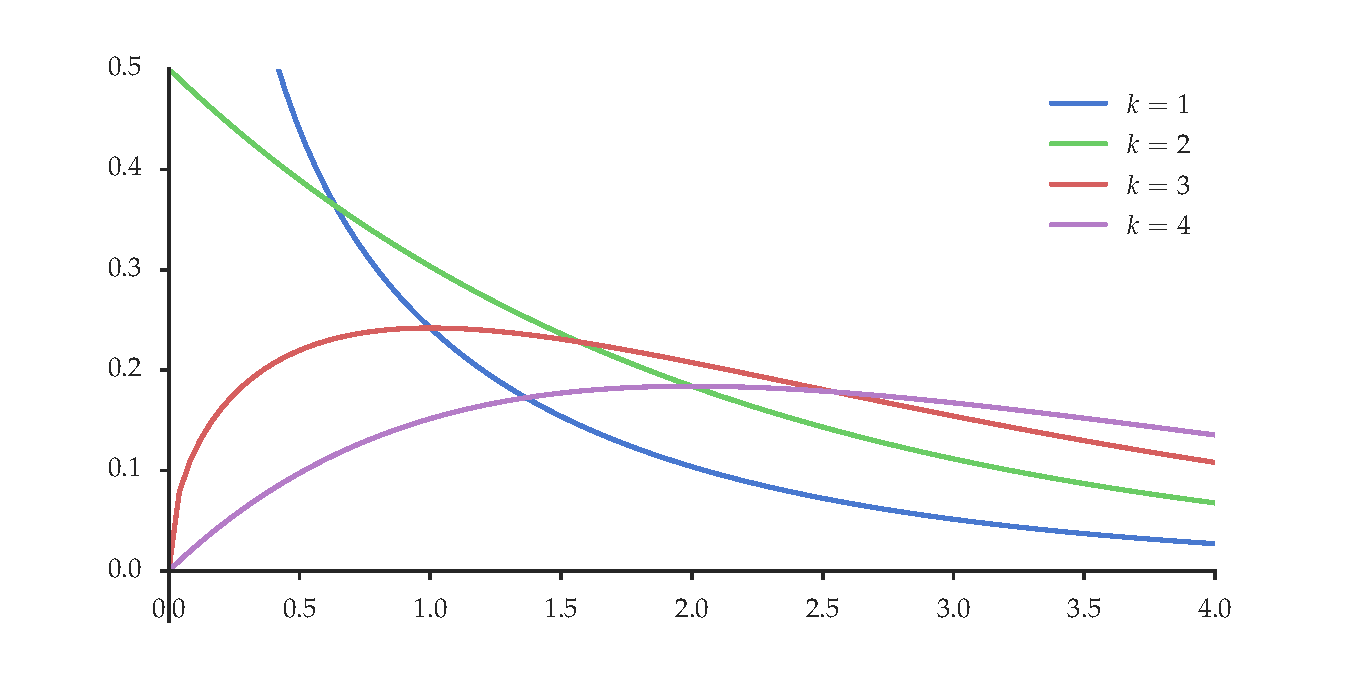
\includegraphics[trim={2em 2em 2em 2em}, clip]{chisq_densities.pdf}}
    \caption{\label{f:chisq_densities} Chi-squared densities}
   \end{center}
    \end{figure}
    
\end{frame}

\begin{frame}

    \vspace{2em}
    \Eg
    \navy{Student's $t$-distribution with $k$ degrees of freedom}, or, more simply,
    the $t$-distribution with $k$ degrees of freedom, is the distribution on $\RR$
    with density
    %
    \begin{equation*}
        p(s) := \frac{\Gamma(\frac{k+1}{2})}{(k\pi)^{1/2} \Gamma(\frac{k}{2})}
        \left( 1 + \frac{s^2}{k} \right)^{-(k+1)/2}
        \qquad (s \in \RR,\; k > 0)
    \end{equation*}
    
\end{frame}

\begin{frame}

    \vspace{2em}
    \Eg
    The \navy{$F$-distribution} with parameters $k_1, k_2$ is the distribution
    with the unlikely looking density
    %
    \begin{equation*}
        p(s) 
        := \frac{\sqrt{(k_1 s)^{k_1}k_2^{k_2}/[k_1 s + k_2]^{k_1 + k_2}}}
            {s B(k_1/2, k_2/2)}
        \qquad (s \geq 0, \; k_1, \, k_2 > 0)
    \end{equation*}
    %
    The $F$-distribution arises in a number of hypothesis tests, as discussed below
    
\end{frame}

\begin{frame}\frametitle{Integrating with Distribution}

    \vspace{2em}
    Consider ordinary integral $\int_a^b
    h(s)\diff s$ of a well-behaved function $h$ on some interval $[a, b]$
    
    Suppose we want to weight this integral, assigning more mass to different regions of
    $[a, b]$: $$\int_a^b h(s) p(s) \diff s$$
    
    For example:
    \begin{itemize}
        \item $h$ as a welfare function and $p$ the density of agents 
        \item $p$ as a density
    indicating probabilities of outcomes, $h$ as a payoff function 
    \end{itemize}

\end{frame}

\begin{frame}

    \vspace{2em}
    Suppose $P$ does not have a density, but we still want to weight using $P$
    \begin{itemize}
        \item we want to define $\int h(s) P(\diff s)$ 
    \end{itemize}
    
    Take distribution $P$ on $\RR$ and consider $(\RR, \bB(\RR), P)$ as a probability space
    
    $(\RR, \bB(\RR), P)$ has its own expectation operator $\EEP $ 
    
    Assume $h$ is a random variable on $(\RR, \bB(\RR), P)$, then
    %
    \begin{equation*}
        \EEP h :=: \int h(s) P(\diff s) 
        := \text{the expectation of $h$ under $P$}
    \end{equation*}
    
\end{frame}

\begin{frame}

    \vspace{2em}
    \Fact
    Let $h \colon \RR \to \RR$ be $\bB$-measurable and let $P$ be a
    distribution on $\RR$
    
    If $P$
    is discrete, with {\sc pmf} $\{p_j\}_{j \geq 1}$ and support
    $\{s_j\}_{j \geq 1}$, then
    %
    \begin{equation*}
        \label{eq:hasp}
        \int h(s) P(\diff s) = \sum_{j\geq 1} h(s_j) p_j 
    \end{equation*}
    %
    If $P$ is absolutely continuous with density $p$, then
    %
    \begin{equation*}
        \label{eq:hasd}
        \int h(s)P(\diff s) = \int_{-\infty}^{\infty} h(s) p(s) \diff s
    \end{equation*}
    %
\end{frame}


\begin{frame}\frametitle{Distributions and Random Variables}

    \vspace{2em}
    Every random
    variable defines a distribution on $\RR$ 
    
    \vspace{.7em}
    Let $x$ be a random variable on some probability space $(\Omega,\fF, \PP)$:
    \begin{itemize}
        \item  probability $\PP\{x \in B\}$ is well-defined
        for every $B \in \bB(\RR)$ (see \eqref{eq:dorv})
        \item  the set function $P$ defined by
            %
            \begin{equation}
                \label{eq:pidox}
                P(B) = \PP\{x \in B\} 
                \qquad (B \in \bB(\RR))
            \end{equation}
            %
            is the \navy{distribution of $x$}
    \end{itemize}
    
\end{frame}

\begin{frame}

    \vspace{2em}
    The  {\sc cdf} corresponding to the distribution $P$ of $x$ satisfies
    %
    \begin{equation}
        \label{eq:deffx}
        F(s) = \PP \{x \leq s\}
        \qquad (s \in \RR)
    \end{equation}
    %
    We write $\lL(x) = F$ to indicate that $F$ represents the distribution of $x$
    
    \vspace{.7em}
    \Fact\eqref{ET-fa:axb}
    If $\lL(x)= F$, then $\PP\{a < x \leq b\} = F(b) - F(a)$ for any $a \leq b$
    
    Proof is an exercise (or see page 111 in ET) 
    
\end{frame}

\begin{frame}

    \vspace{2em}
    For every {\sc cdf} $F$, there exists a probability
    space $(\Omega, \fF, \PP)$ and a random variable $x \colon \Omega \to \RR$
    such that $\lL(x) = F$;  \S\ref{ET-ss:it} outlines one construction
    
\end{frame}

\begin{frame}
    
    \vspace{2em}
    If $\lL(x) = P$ and $P$ has density $p$, we say
    \navy{$x$ has density $p$}
    
    If the distribution of $x$ is discrete, we'll call
    $x$ a \navy{discrete random variable}
    
    \vspace{1em}
    \Fact
    If $x$ has a density, then $\PP\{x=s\}=0$ for all $s \in \RR$, and for
    any $a < b$,
    %
    \begin{multline*}
        \PP\{a < x < b\}
        = \PP\{a < x \leq b\}
        \\ = \PP\{a \leq x < b\}
        = \PP\{a \leq x \leq b\}
    \end{multline*}
    %
\end{frame}

\begin{frame}\frametitle{Distributions of Transformations}

    \vspace{2em}
    \Fact\eqref{ET-fa:cdftr}
    If $\lL(x) = F$ and $y := \psi(x)$, where $\psi \colon \RR \to \RR$ is
    strictly increasing, then $\lL(y)= G$ where $G(s) := F(\psi^{-1}(s))$.
    
    \Prf
    Observe under these hypotheses $\psi^{-1}$ exists and is
    (weakly) increasing.  Hence 
    %
    \begin{equation*}
        \PP\{y \leq s\} 
        = \PP\{\psi(x) \leq s\} 
        = \PP\{x \leq \psi^{-1}(s) \} 
        = F( \psi^{-1}(s) )
    \end{equation*}
    %
    Note how monotonicity is used in the second equality

\end{frame}

\begin{frame}

    \vspace{2em}
    \Eg
    If $\lL(x) = F$ and $y := \exp(x)$, then the {\sc cdf} of $y$ is $G(s) := F(\ln(s))$
    
\end{frame}

\begin{frame}

    \vspace{2em}
    \Fact\eqref{ET-fa:trden}
    If $x$ has density $p$ on $\RR$ and $y := \psi(x)$ where $\psi$ is a
    diffeomorphism on $\RR$, then the distribution of $y$ is absolutely
    continuous, with density
    %
    \begin{equation*}
        \label{eq:trden}
        q(s) = p(\psi^{-1}(s)) \left| \frac{\diff \psi^{-1}(s)}{\diff s} \right|
                 \qquad (s \in \RR)
    \end{equation*}
    
    
    \vspace{1em}
    The term \navy{diffeomorphism} means  $\psi$ is a bijection on
    $\RR$ and both $\psi$ and its inverse are differentiable
    
\end{frame}

\begin{frame}

    \vspace{2em}
    \Eg
    If $x$ has density $p$ on $\RR$ and $\mu$ and $\sigma$ are constants with 
    $\sigma > 0$, then the density of $y := \mu + \sigma x$ is
    %
    \begin{equation*}
        q(s) = p \left( \frac{s - \mu}{\sigma} \right) 
                 \frac{1}{\sigma} 
                 \qquad (s \in \RR)
    \end{equation*}
    %
    When $x$ is standard normal: $y = \mu
    + \sigma x$ is $\nN(\mu, \sigma^2)$
    
    Why?
    \begin{itemize}
        \item Take $p$ to be the standard normal density $\phi$
        \item Recall%
            \begin{equation*}
                p(s) = F'(s) = 
                \frac{1}{\sqrt{2 \pi} \sigma}
                   \exp \left\{ - 
                       \frac{(s - \mu)^2}{2\sigma^2} \right\} 
            \end{equation*}
    %
    \end{itemize}
    
\end{frame}

\begin{frame}

    \vspace{2em}
   Let $x$ be a random variable on probability space $(\Omega, \fF, \PP)$
   
   The distribution of $x$ encodes all information to calculate 
   expectations of $x$ or of any $\bB$-measurable transformation $h(x)$
   
   First, let $x$ be finite. Suppose 
   
   \begin{itemize}
       \item  $\lL(x) = P$
       \item  the function $h\colon \RR \to \RR$ is any $\bB$-measurable function
       \item $P$ puts all mass on finite set $\{s_j\}_{j=1}^J$
   \end{itemize}
   
   \vspace{.7em}
   Using $\PP\{x = s_j\} = P\{s_j\}$ and the definition of expectations:
   %
    \begin{equation*}
        \label{eq:ehx}
        \EE h(x) 
        = \sum_{j=1}^J h(s_j) \PP\{x = s_j\}
        = \sum_{j=1}^J h(s_j) P\{s_j\}
        = \sum_{j=1}^J h(s_j) p_j
    \end{equation*}

\end{frame}

\begin{frame}
       
    \vspace{2em}
   The expectation of $h(x)$ on $(\Omega, \fF, \PP)$  equal to the 
   expectation of $h$ on $(\RR, \bB(\RR), P)$
   
   True also for the infinite case:
   
   \vspace{1em}
   \Fact
    Let $x$ be a random variable on some probability space $(\Omega, \fF,
    \PP)$, let $\lL(x) = P$ and let $h$ be a $\bB$-measurable function such
    that $h(x)$ is integrable. The expectation $\EE h(x)$ is entirely
    determined by $h$ and $P$.  In particular,
    %
    \begin{equation*}
        \EE h(x) = \int h(s) P(\diff s)
    \end{equation*}
    %
    where $\int h(s) P(\diff s)$ is the expectation of $h$ on $(\RR, \bB(\RR), P)$

\end{frame}

\begin{frame}

    \vspace{2em}
    \Eg
    Let $x$ be a random variable whose distribution $P$ is the uniform
    distribution on $[a, b]$
    
    \vspace{.7em}
    Apply the definition of the uniform density
    %
    \begin{equation*}
        \EE x 
        = \int s P(\diff s) 
        = \int s p(s) \diff s 
        = \int_{-\infty}^{\infty} 
         \frac{s}{b - a} \1\{a \leq s \leq b\} \, \diff s 
    \end{equation*}
    %
    Solving the integral gives $\EE x = \mu := (a + b)/2$.  The variance is 
    %
    \begin{multline*}
        \var [x]
        = \int (s - \mu)^2 P(\diff s)
        \\ = \int_a^b
            \left(s -\frac{a + b}{2} \right)^2
            \frac{1}{b - a} \diff s
        = \frac{1}{12} (b-a)^2
    \end{multline*}
    
\end{frame}



\begin{frame}

    \vspace{2em}
    \Eg
    Suppose  $\lL(x) = \nN(\mu, \sigma)$
    
    If $\sigma > 0$, the mean can be computed via
    %
    \begin{equation*}
        \EE x 
        = \int_{-\infty}^{\infty} s 
        \frac{1}{\sqrt{2 \pi} \sigma}
           \exp \left\{ - 
               \frac{(s - \mu)^2}{2\sigma^2} \right\}  \diff s
        = \mu
    \end{equation*}
    %
    The variance is given by:
    %
    \begin{equation*}
        \var [x]
        = \int_{-\infty}^{\infty}
            (s - \mu)^2
            \frac{1}{\sqrt{2 \pi} \sigma}
               \exp \left\{ - 
               \frac{(s - \mu)^2}{2\sigma^2} \right\}  \diff s
        = \sigma^2
    \end{equation*}
    
\end{frame}

\begin{frame}\frametitle{Moments from Distributions}

    \vspace{2em}
    Any two random variables with the same
    distribution share the same moments
    
    Hence moments are best thought of as a
    property of the distribution, not the random variable
    
    \vspace{.7em}
    Thus we define 
    %
    \begin{itemize}
        \item the \navy{mean} of $P$ as $\mu = \int s P(\diff s)$,
        \item the \navy{$k$th moment} of $P$ as $\int s^k P(\diff s)$, 
        \item the \navy{variance} of $P$ as $\int (s - \mu)^2 P(\diff s)$,
    \end{itemize}
    %
    and so on

\end{frame}

\begin{frame}\frametitle{Quantile Function}

    \vspace{2em}
    Let $F$ be a strictly increasing {\sc cdf} on $\RR$
    
    Given $\tau \in (0, 1)$, the \navy{$\tau$th quantile} of $F$ is the $\xi \in \RR$ that solves $F(\xi) = \tau$
    
    Under our assumptions on $F$, such a $\xi$ exists and is uniquely defined
    
    The $0.5$th quantile is called the \navy{median} of $F$

\end{frame}

\begin{frame}

    \vspace{2em}
    The \navy{quantile function}:
    %
    \begin{equation*}
        \label{eq:quantwi}
        F^{-1}(\tau) := \text{ the unique } \xi \text{ such that } F(\xi) = \tau
        \qquad (0 < \tau < 1)
    \end{equation*}
    
    
    \vspace{.7em}
    \Eg
    The quantile function associated with the standard Cauchy distribution  
    is $F^{-1}(\tau) = \tan [\pi(\tau - 1/2)]$

\end{frame}

\begin{frame}

    \begin{figure}
   \begin{center}
    \scalebox{.44}{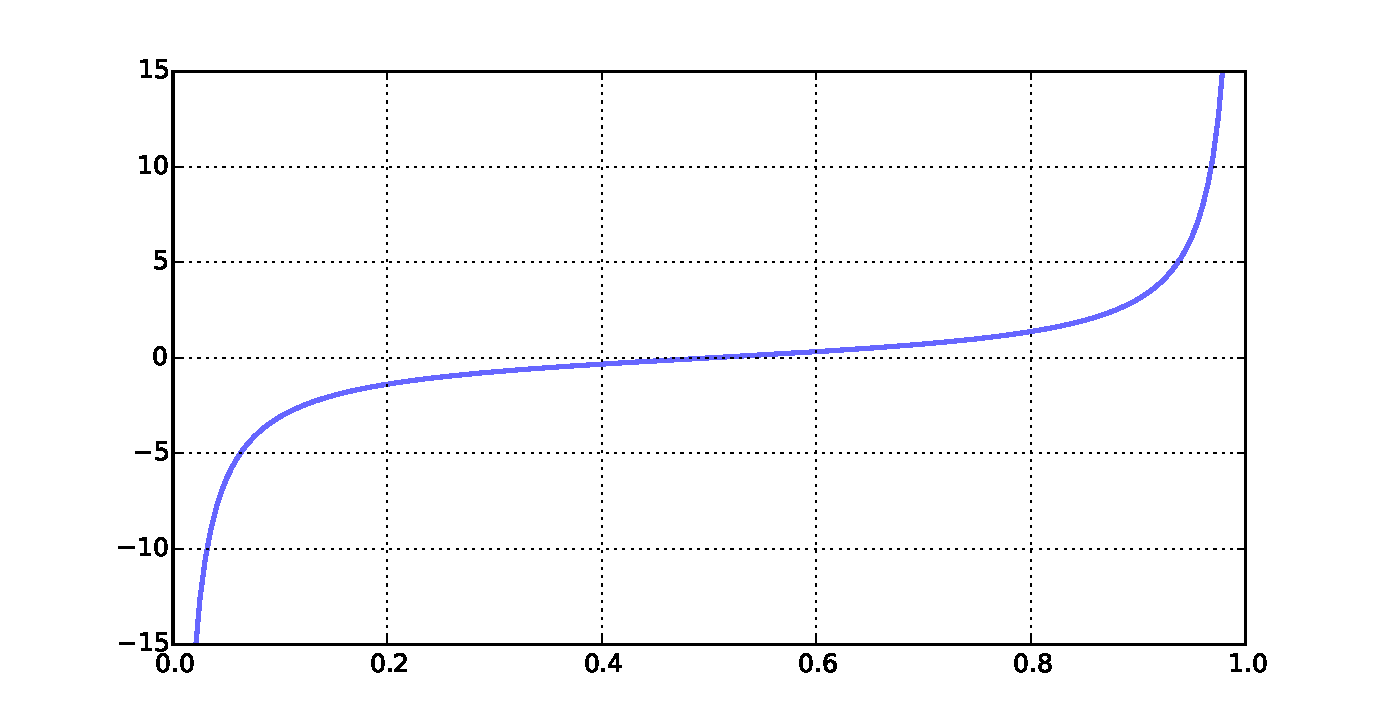
\includegraphics[trim={0 0em 0 2em}, clip]{cauchy_quant.pdf}}
    \caption{\label{f:cauchy_quant} Cauchy quantile function (The horizontal axis is $\tau \in
    (0, 1)$)}
   \end{center}
\end{figure}

\end{frame}

\begin{frame}

    \vspace{2em}
    When $F$ is not strictly increasing, $F^{-1}$ not well-defined
    
    \vspace{1em}
    We can set:
    %
    \begin{equation}
        \label{eq:quantwi2}
        F^{-1}(\tau) := \inf \setntn{s \in \RR}{F(s) \geq \tau}
        \qquad (0 < \tau < 1)
    \end{equation}
    %
\end{frame}

\begin{frame}

    \vspace{2em}
    A density $p$ is symmetric if $p(s) = p(-s)$ for all $s \in \RR$
    
    A common scenario in hypothesis testing 
    
    \vspace{.7em}
    \Fact\eqref{ET-fa:avsc}
    Let $x$ be a random variable with density $p$.  If $p$ is symmetric, then
    the {\sc cdf} $G$ of $y := |x|$ is given by 
    %
    \begin{equation*}
        G (s) 
        := \PP\{y\leq s\} 
        = 
        \begin{cases}
            2 F(s) - 1 & \text{ if } s \geq 0
            \\
            0 & \text{ otherwise}
        \end{cases}
    \end{equation*}
    %
    Proof as exercise \ref{ET-ex:avsc}
    
    Fact equivalent to $F(s) = 1 - F(-s)$

\end{frame}

\begin{frame}

    \vspace{2em}
    Take a random variable $x$ with $\lL(x) = F$ and constant $\alpha \in
    (0,1)$ as given
    
    \vspace{.7em}
    Consider the $c$ that solves $\PP\{-c \leq x \leq c \}  =
    1 - \alpha$
    
    \Fact
        If $\lL(x) = F$, $x$ has a symmetric density and $F$ is strictly increasing, then
        %
        \begin{equation}
            \label{eq:symcdf}
            c = F^{-1}(1 - \alpha/2) 
            \quad \implies \quad
            \PP\{-c \leq x \leq c\} = 1 - \alpha
        \end{equation}
        %
    When $F$ is the standard normal {\sc cdf} $\Phi$, $c$ is usually denoted by $z_{\alpha/2}$:
    %
    \begin{equation}
        \label{eq:zalpha2}
        z_{\alpha/2} := \Phi^{-1}(1 - \alpha/2)
    \end{equation}
    
\end{frame}

\begin{frame}

    \begin{figure}
   \begin{center}
    \scalebox{.44}{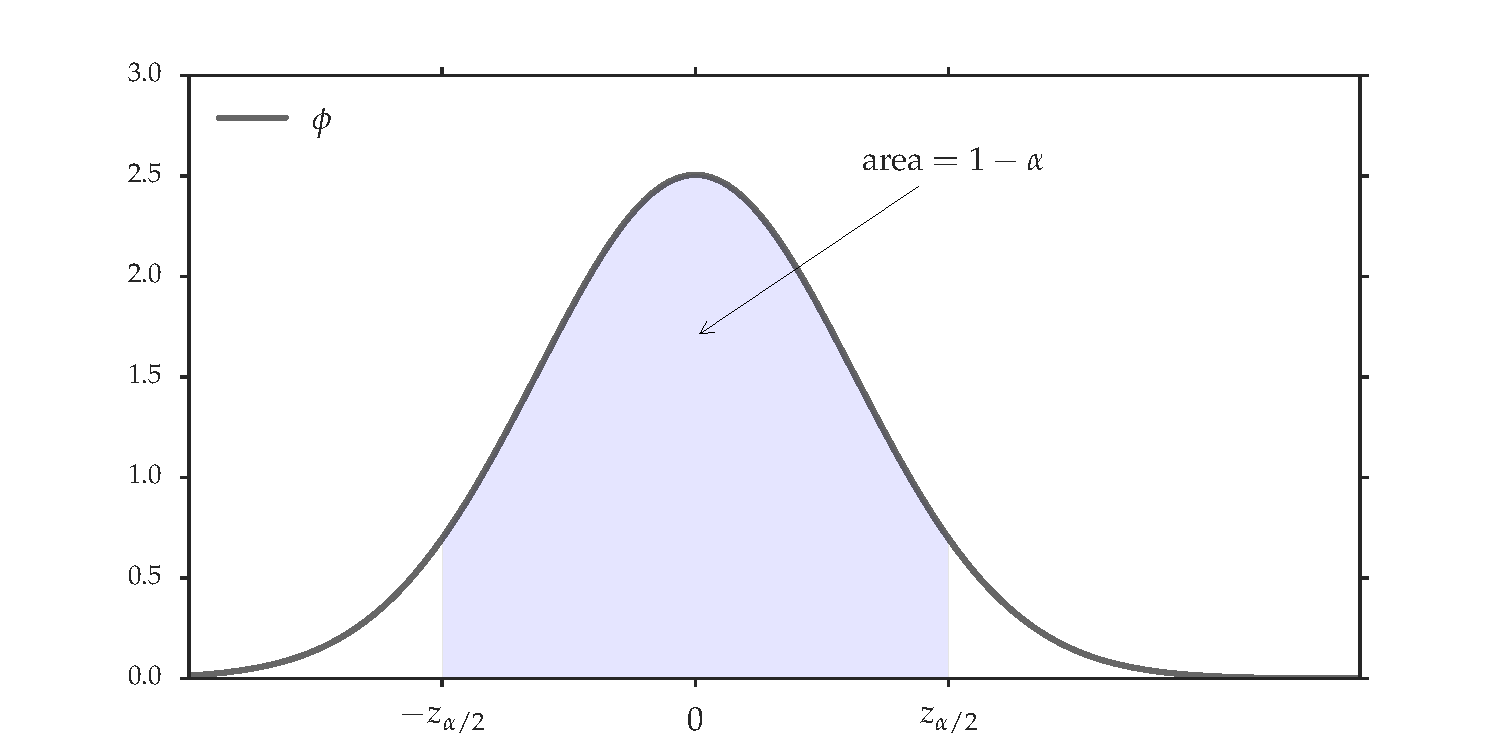
\includegraphics[trim={2em 2em 2em 2em}, clip]{fcca.pdf}}
    \caption{\label{f:fcca} Critical values for the standard normal density}
   \end{center}
    \end{figure}

\end{frame}


\end{document}
